% Лабораторная работа по АСиСу № 11
% Михедов Константин Константинович

% Тип документа: статья, на бумаге А4
\documentclass[a4paper]{article}

% Подключение сторонних tex файлов 
\usepackage{import}


% Основные данные - ВУЗ, факультет, город...
\import{./../../stuff/tex}{config.tex}

% Подключение необходимых зависимостей
\import{./../../stuff/tex/settings}{packages.tex}
% Настройка подключенных пакетов
\import{./../../stuff/tex/settings}{preferences.tex}


% Шаблон титульной страницы 
\import{./../../stuff/tex/templates}{title.tex}
% Упрощенный блок "выполнил"
\import{./../../stuff/tex/templates}{sign1.tex}
% Макрос для содержания
\import{./../../stuff/tex/templates}{toc.tex}

% Определяем название документа
\title{
  Лабораторная работа №11 по курсу \\
  <<Компьютерный практикум <<Администрирование систем и сетей>>  
}
% Отключаем отображение правительства
\renewcommand{\government}{}
% Отключаем сокращенное нзавание университета
\renewcommand{\subuniversity}{}
% Указываем преподавателя
\renewcommand{\shortteachername}{Степанянц В.Г.}


% Путь до внешних изображений
\graphicspath{ {./figures/}}


% Основной текст работы
\begin{document}
  \templatedtitlepage
  
  \toc
  \section{Ход работы}

  Все имена выбраны в соответсвии с 9 вариантом.

  Действия выполняются на виртуальной машине с \textit{Windows Server 2016}.
  Для нее заданы пароль для учетной записи администратора и следующие сетевые настройки:

  \begin{figure}[H]
    \centering
    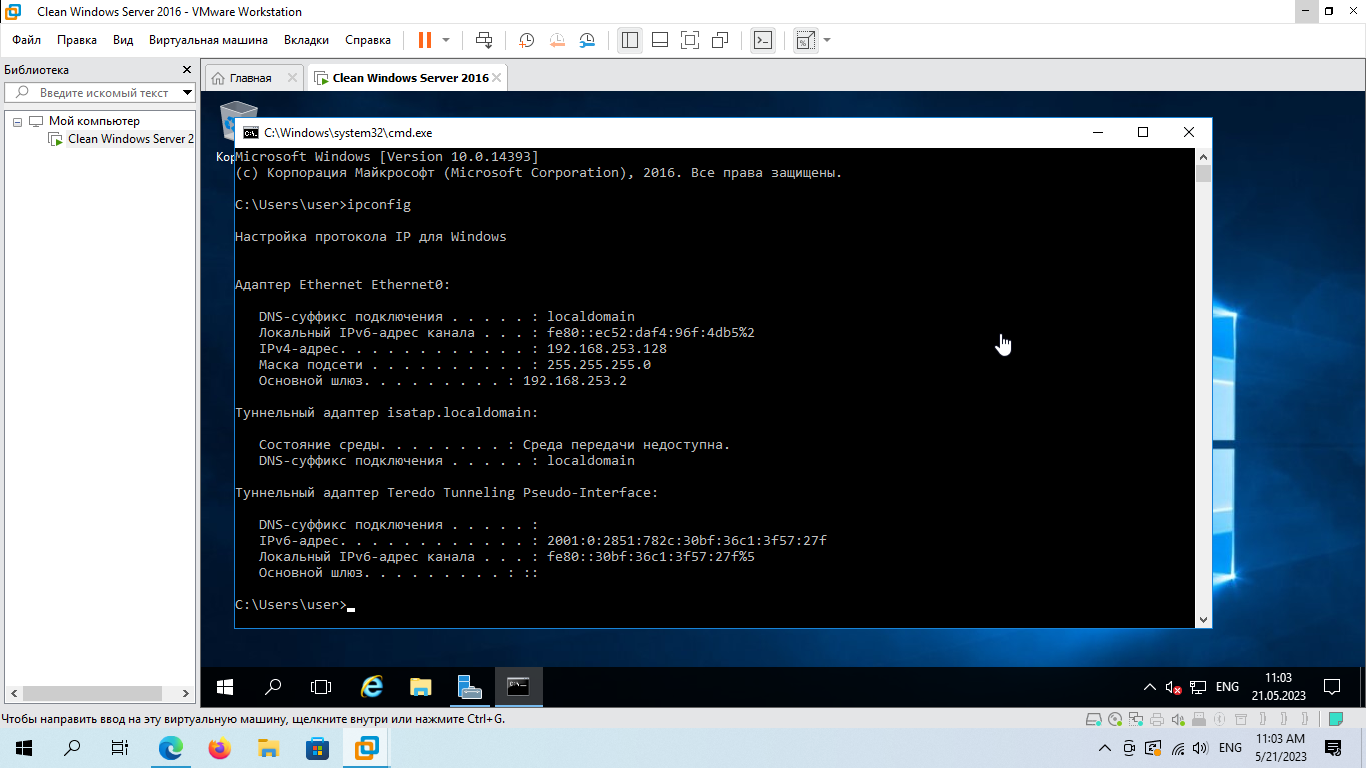
\includegraphics[width=\textwidth]{11_0001}
    \label{img:1}
    \caption{\textit{ipconfig}}
  \end{figure}

  Данная машина подключена к сети 192.168.253.0/24 и имеет \textit{IPv4} адрес
  192.168.253.128 (также настроен шлюз по умолчанию - 192.168.253.2).

  \subsection{Установка необходимых компонентов}

  \begin{figure}[H]
    \centering
    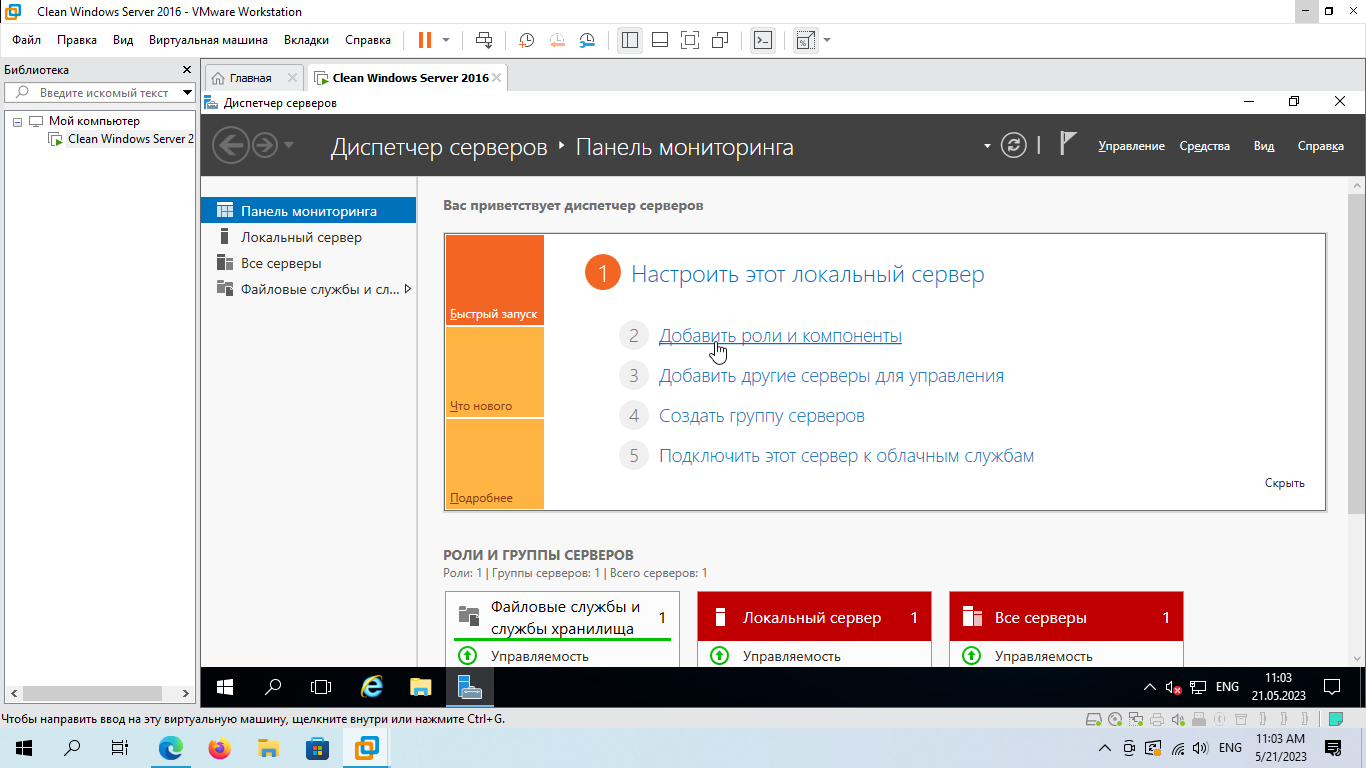
\includegraphics[width=\textwidth]{11_0002}
    \label{img:2}
    \caption{Начинаем добавление ролей и компонентов}
  \end{figure}

  \begin{figure}[H]
    \centering
    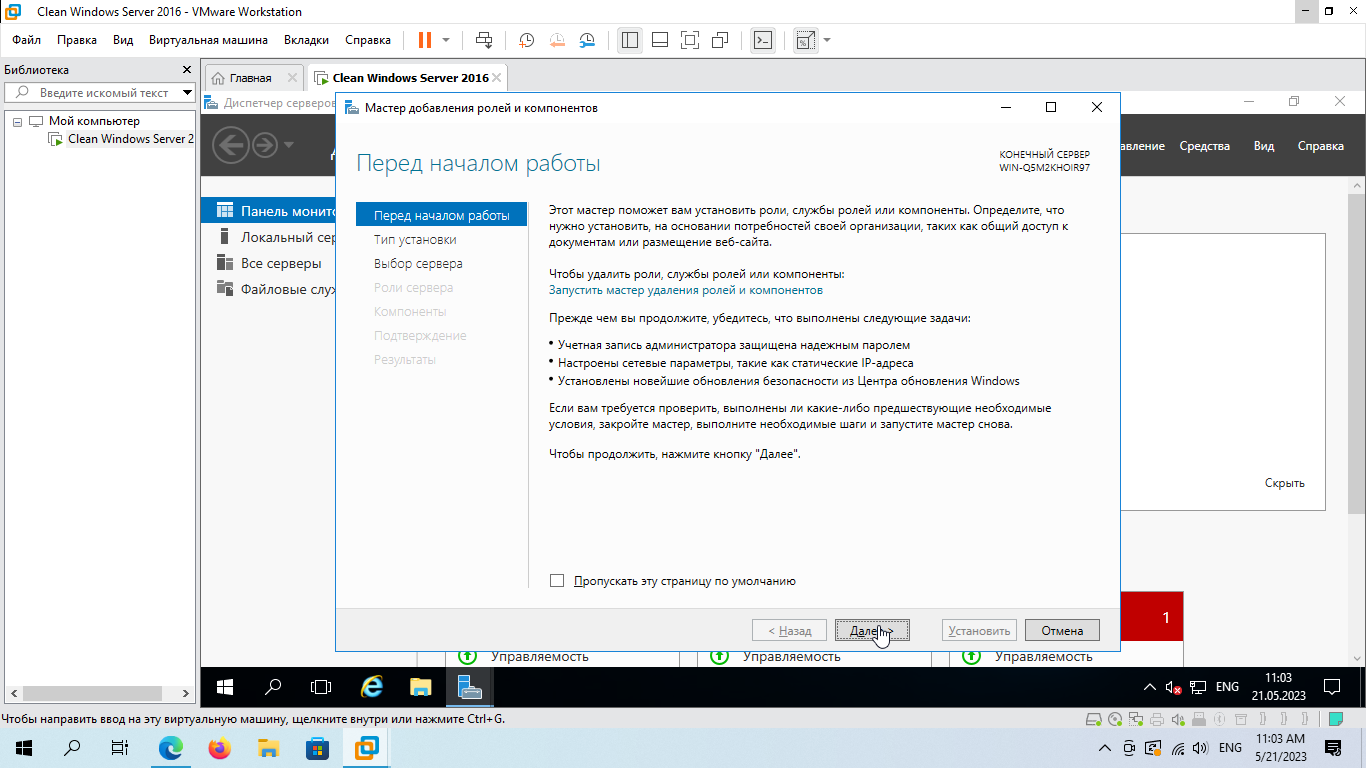
\includegraphics[width=\textwidth]{11_0003}
    \label{img:3}
    \caption{Далее}
  \end{figure}

  \begin{figure}[H]
    \centering
    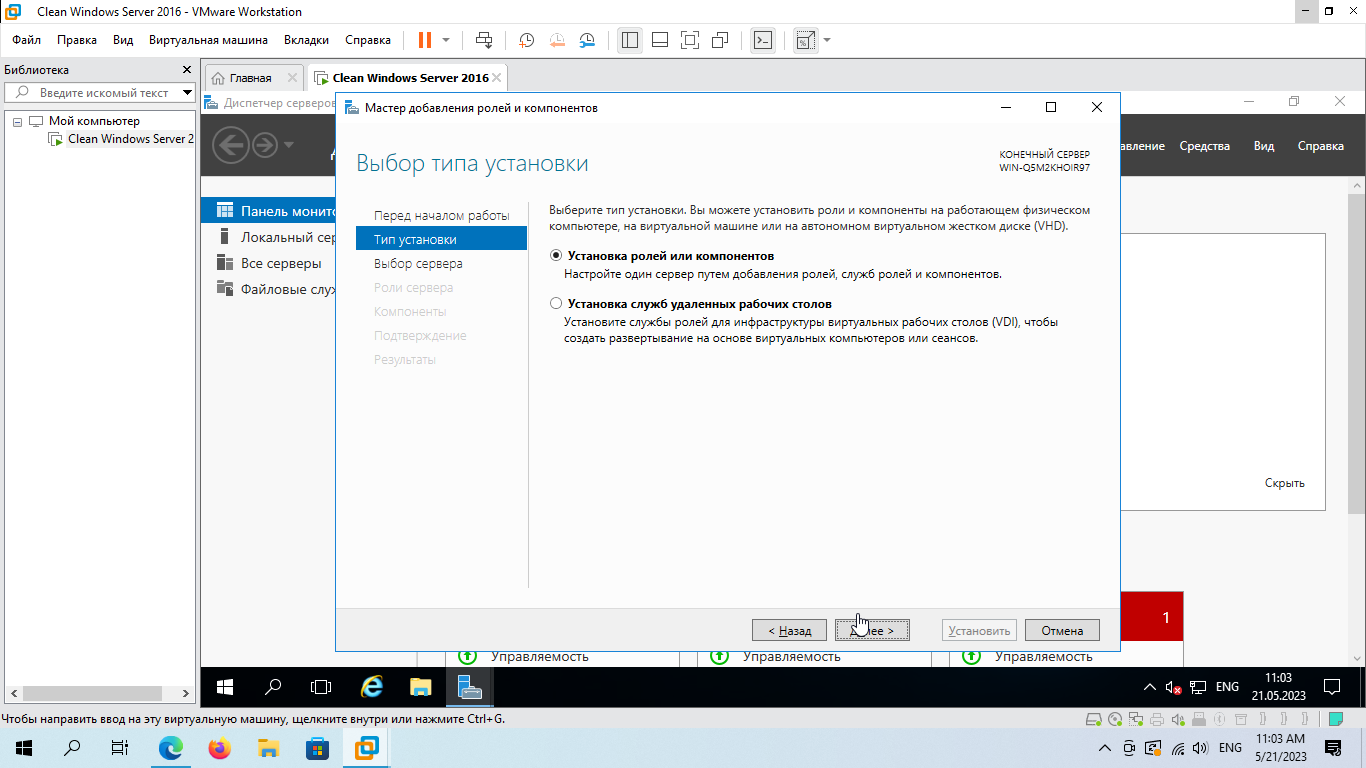
\includegraphics[width=\textwidth]{11_0004}
    \label{img:4}
    \caption{Необходимы роли и компоненты}
  \end{figure}

  \begin{figure}[H]
    \centering
    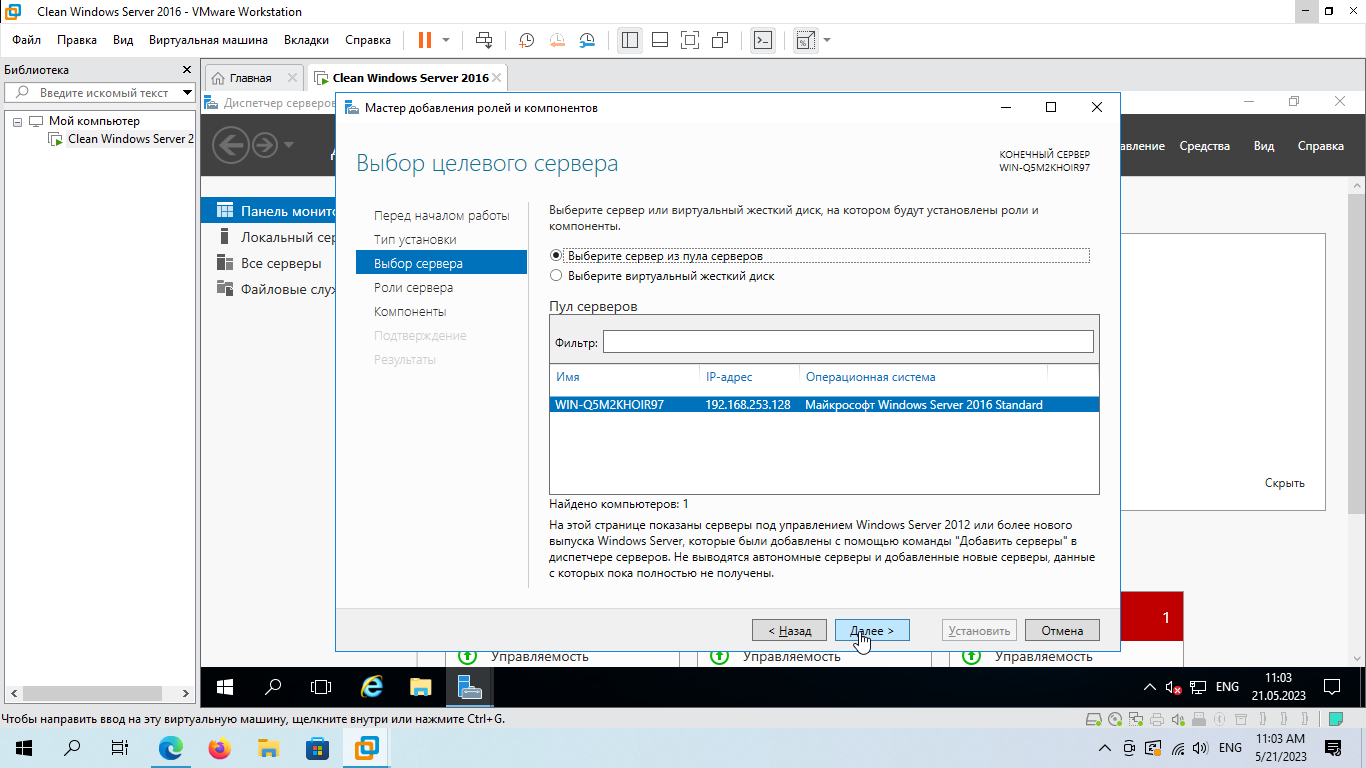
\includegraphics[width=\textwidth]{11_0005}
    \label{img:5}
    \caption{Установка для текущего компьютера}
  \end{figure}

  \begin{figure}[H]
    \centering
    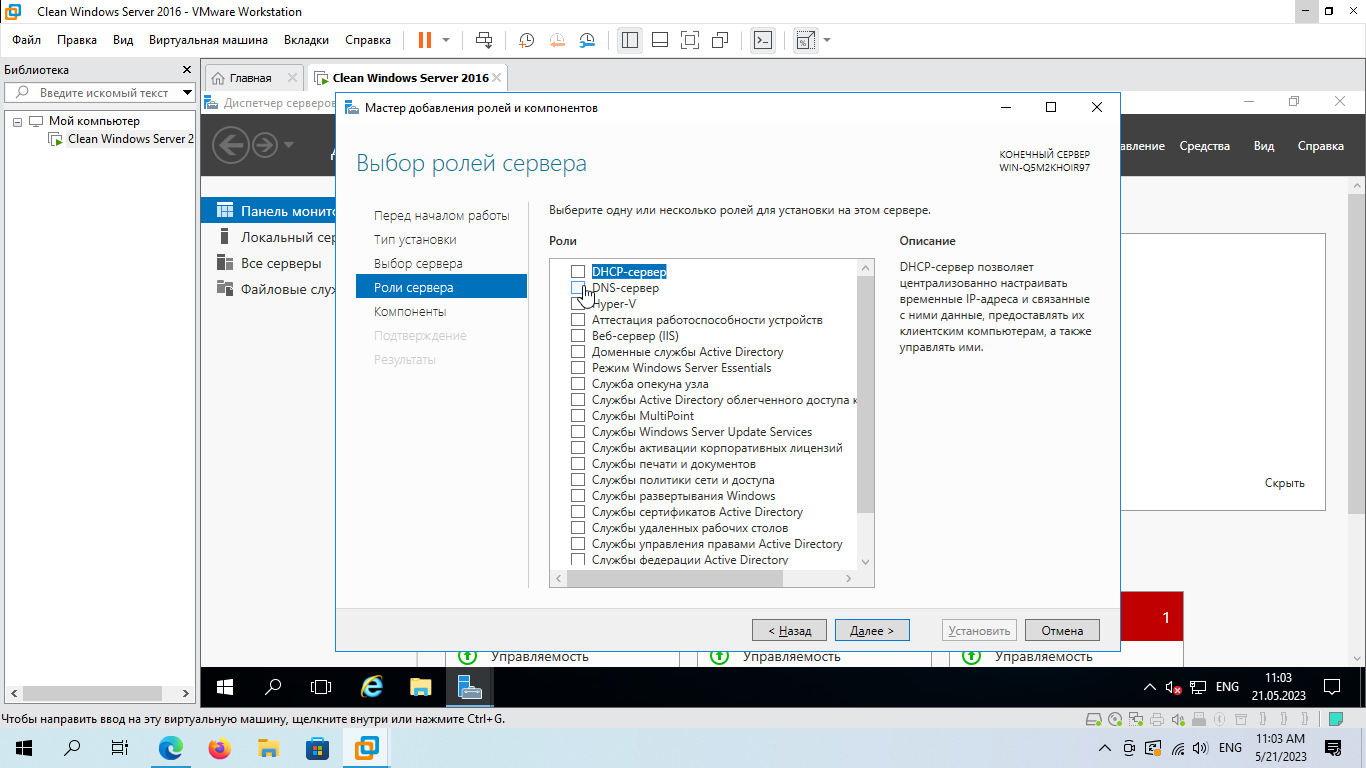
\includegraphics[width=\textwidth]{11_0006}
    \label{img:6}
    \caption{Добавляем роль DNS сервера}
  \end{figure}

  \begin{figure}[H]
    \centering
    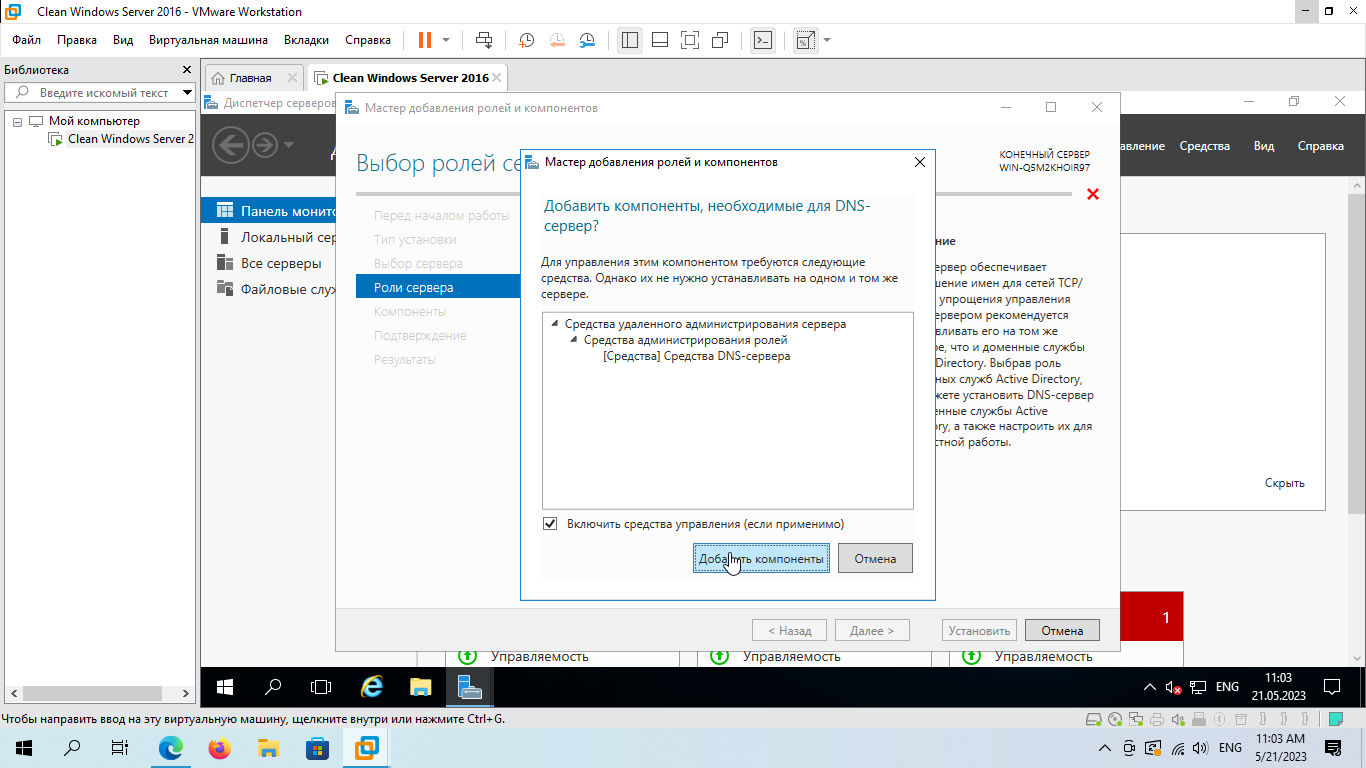
\includegraphics[width=\textwidth]{11_0007}
    \label{img:7}
    \caption{И необходимые для DNS компоненты}
  \end{figure}

  \begin{figure}[H]
    \centering
    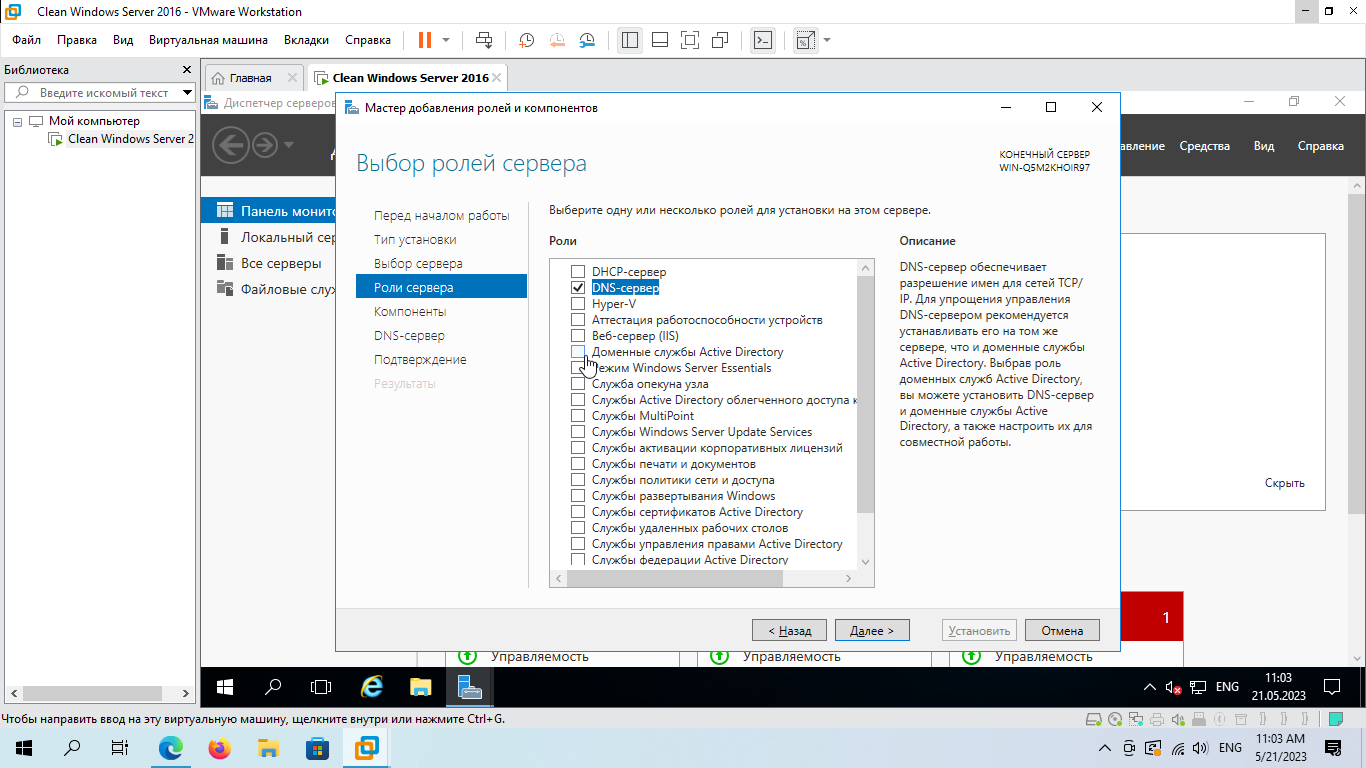
\includegraphics[width=\textwidth]{11_0008}
    \label{img:8}
    \caption{Добавляем роль доменных служб AD}
  \end{figure}

  \begin{figure}[H]
    \centering
    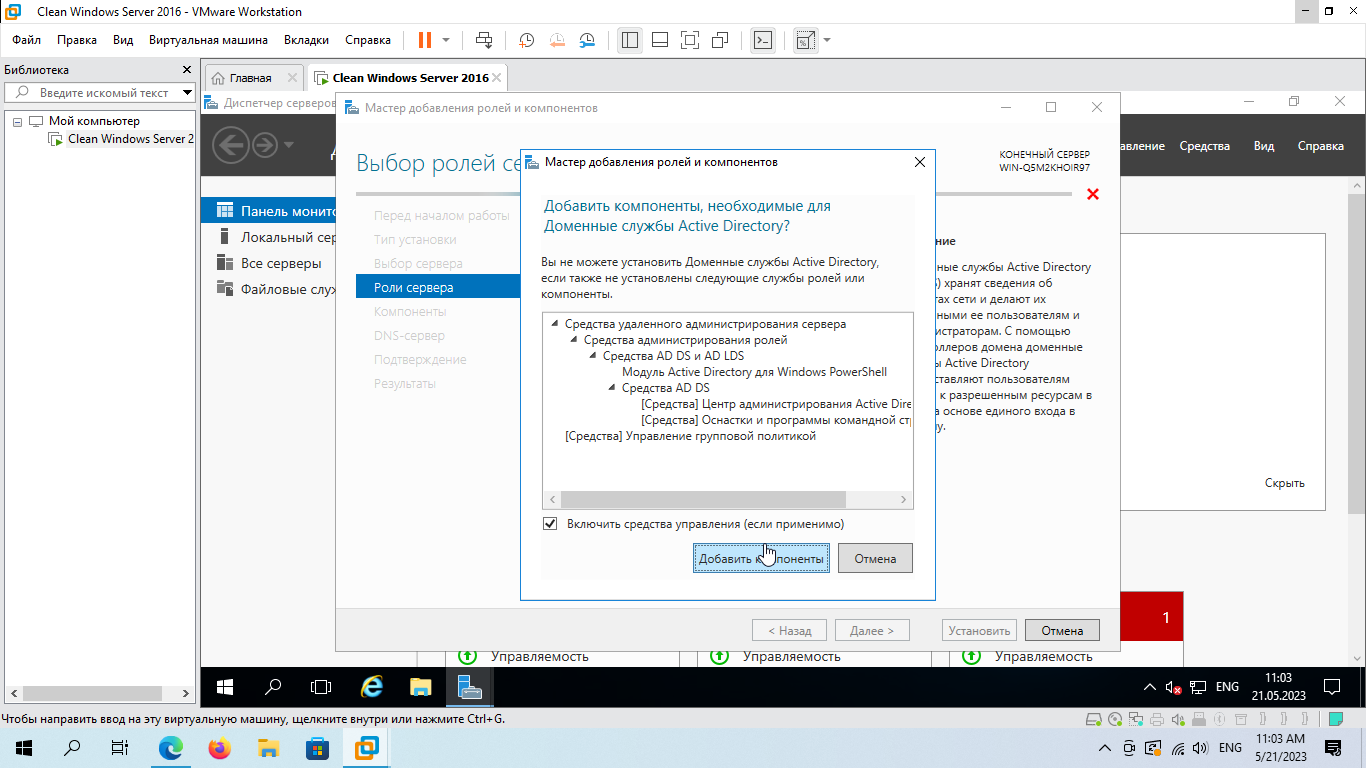
\includegraphics[width=\textwidth]{11_0009}
    \label{img:9}
    \caption{И необходимые для AD компоненты}
  \end{figure}

  \begin{figure}[H]
    \centering
    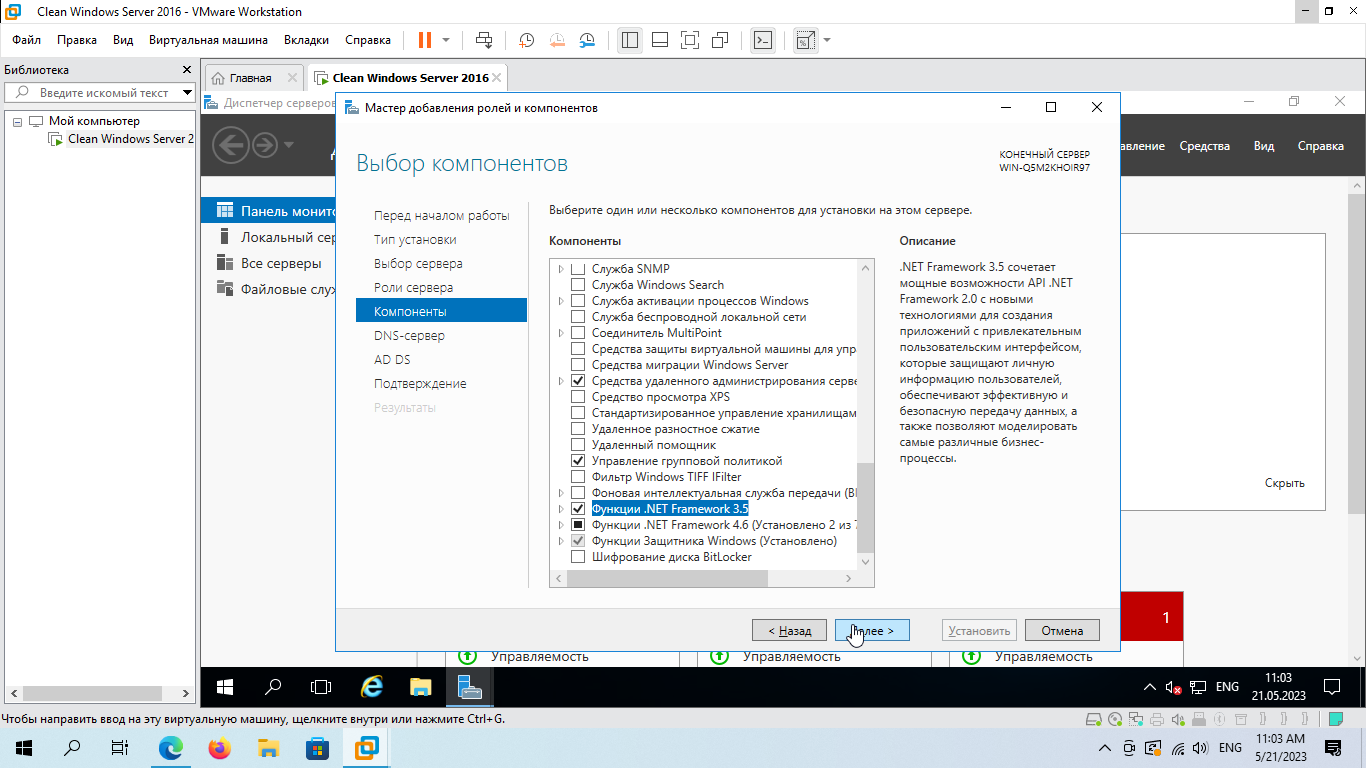
\includegraphics[width=\textwidth]{11_0011}
    \label{img:11}
    \caption{Добавляем новый компонент - .NET Framework 3.5}
  \end{figure}

  \begin{figure}[H]
    \centering
    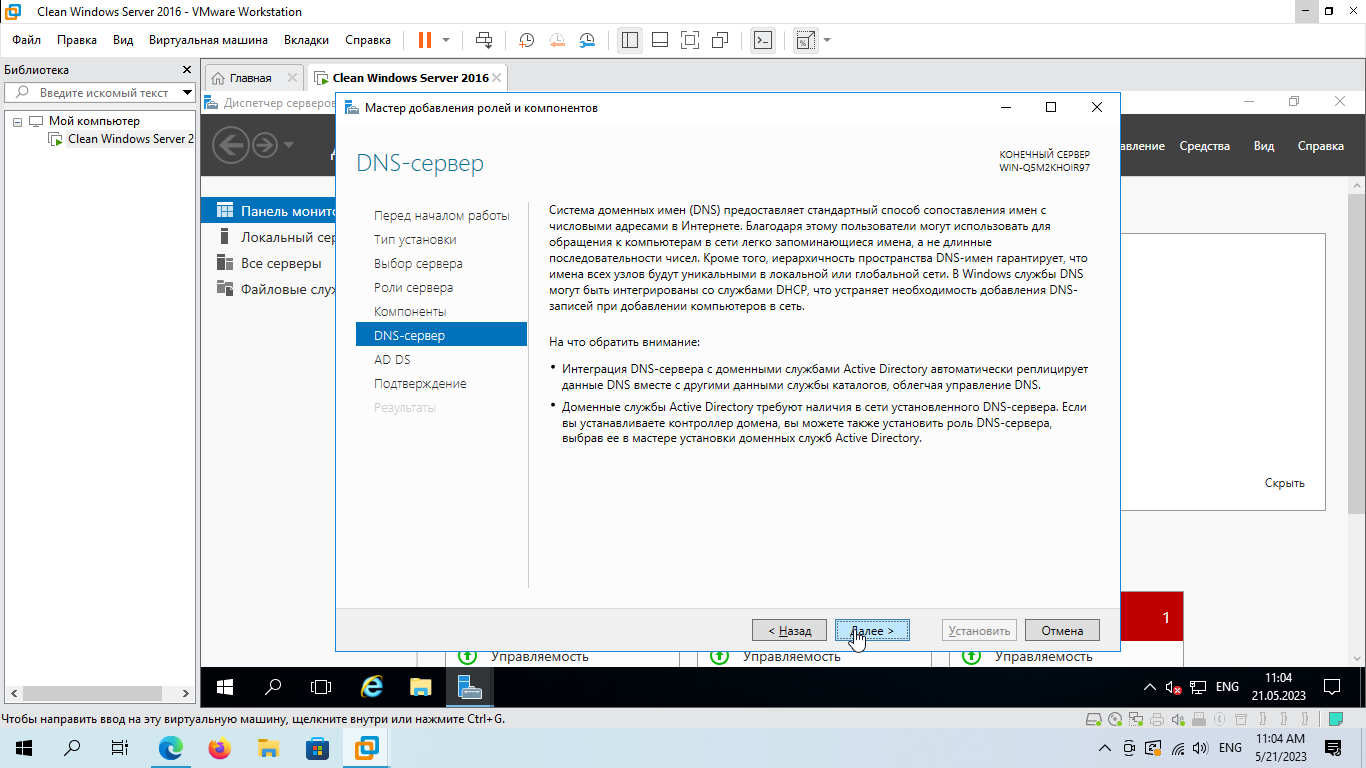
\includegraphics[width=\textwidth]{11_0012}
    \label{img:12}
    \caption{Далее}
  \end{figure}

  \begin{figure}[H]
    \centering
    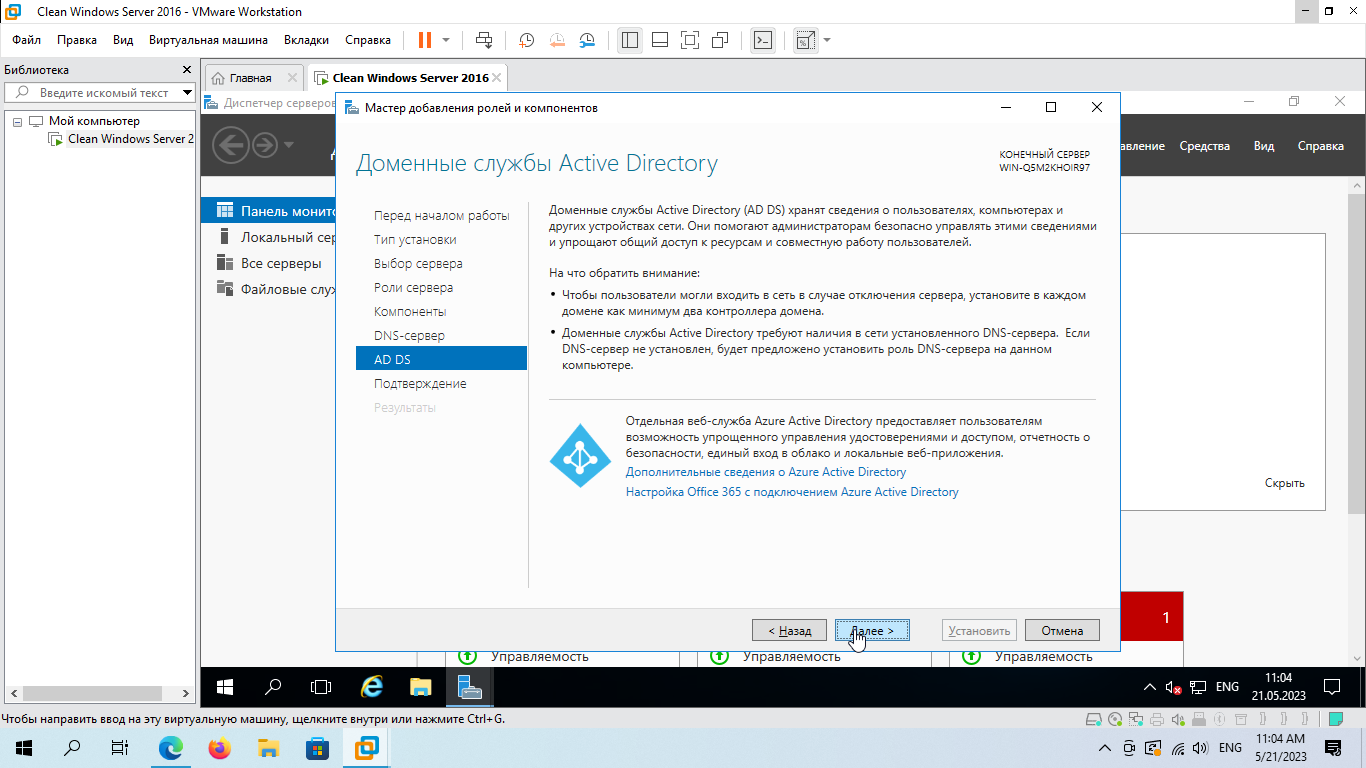
\includegraphics[width=\textwidth]{11_0013}
    \label{img:13}
    \caption{Далее}
  \end{figure}

  \begin{figure}[H]
    \centering
    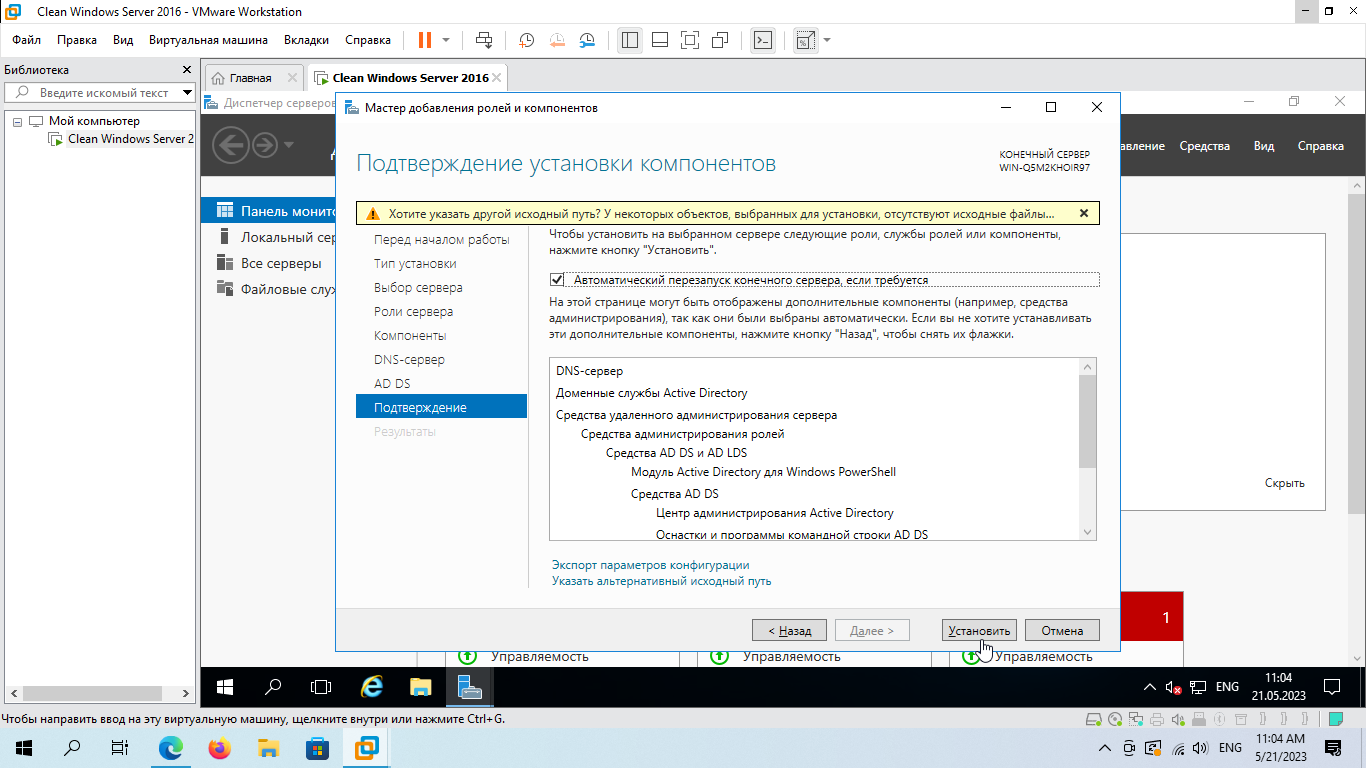
\includegraphics[width=\textwidth]{11_0014}
    \label{img:14}
    \caption{Начинаем установку}
  \end{figure}

  \begin{figure}[H]
    \centering
    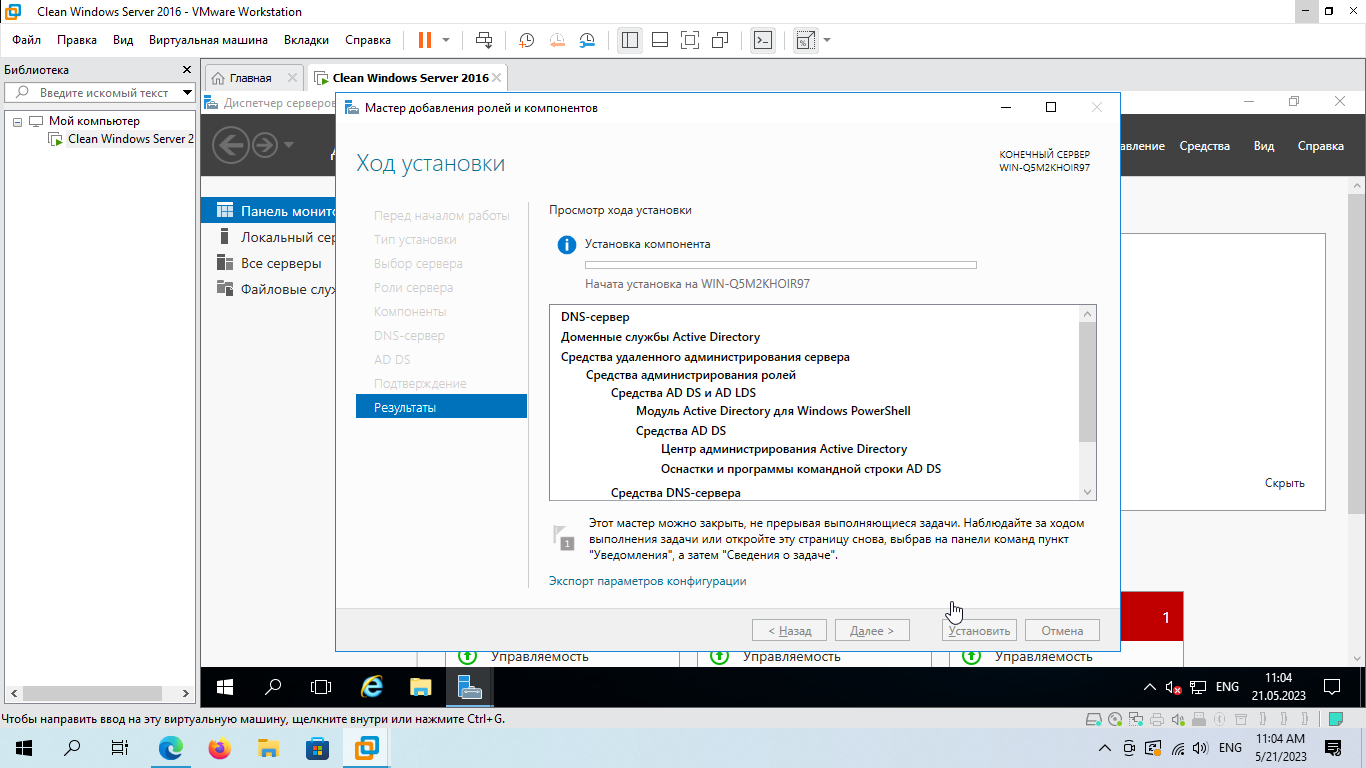
\includegraphics[width=\textwidth]{11_0015}
    \label{img:15}
    \caption{Процесс установки}
  \end{figure}

  Пока происходит установка системных компонентов, произведем ручную
  установку дополнительного программного обеспечения:

  \begin{figure}[H]
    \centering
    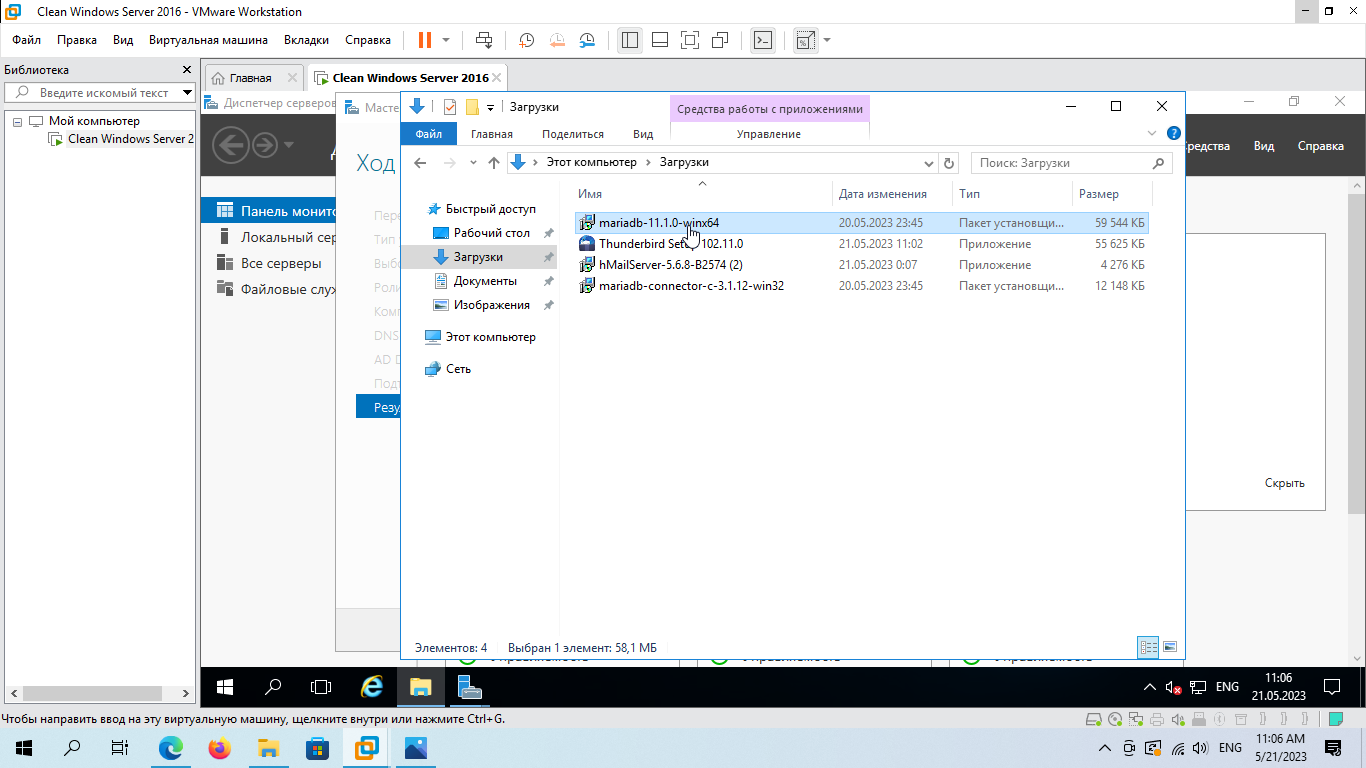
\includegraphics[width=\textwidth]{11_0016}
    \label{img:16}
    \caption{Установим MariaDB}
  \end{figure}

  \begin{figure}[H]
    \centering
    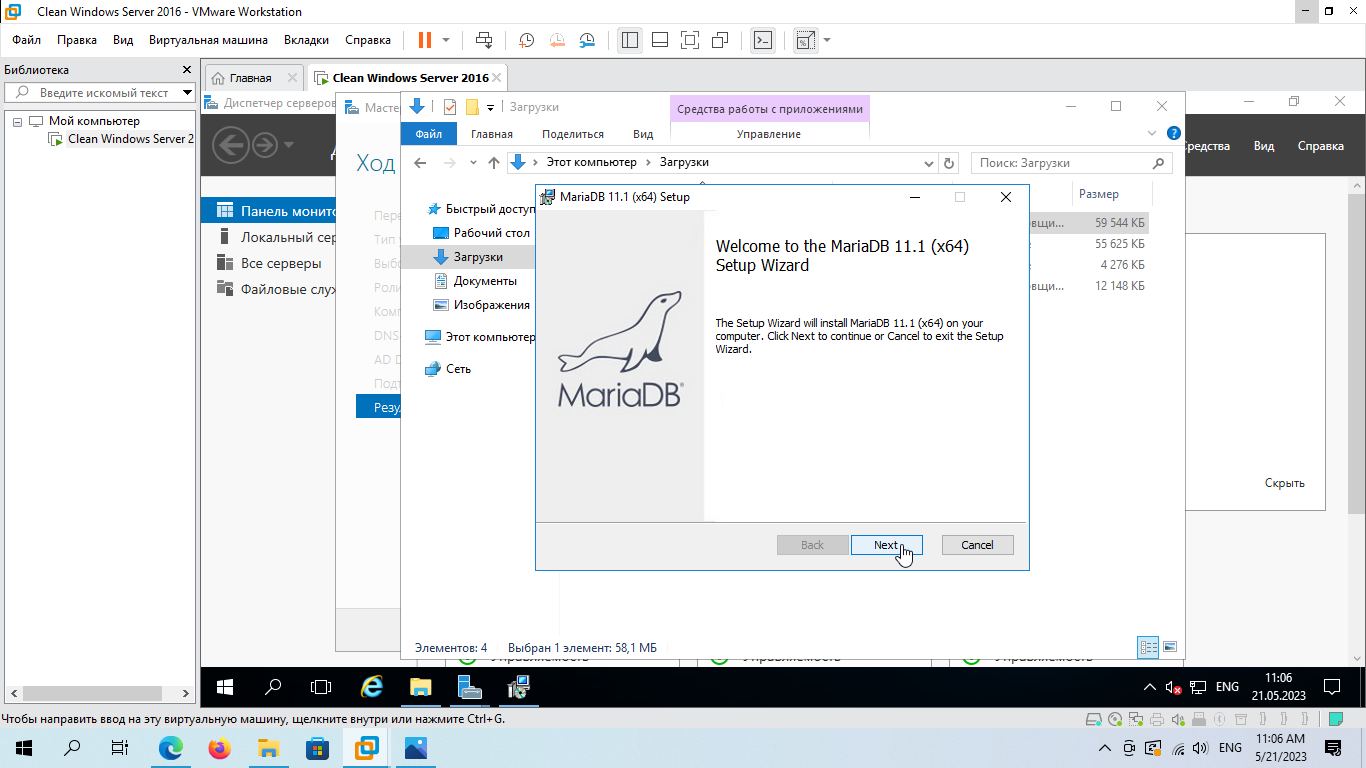
\includegraphics[width=\textwidth]{11_0017}
    \label{img:17}
    \caption{Далее}
  \end{figure}

  \begin{figure}[H]
    \centering
    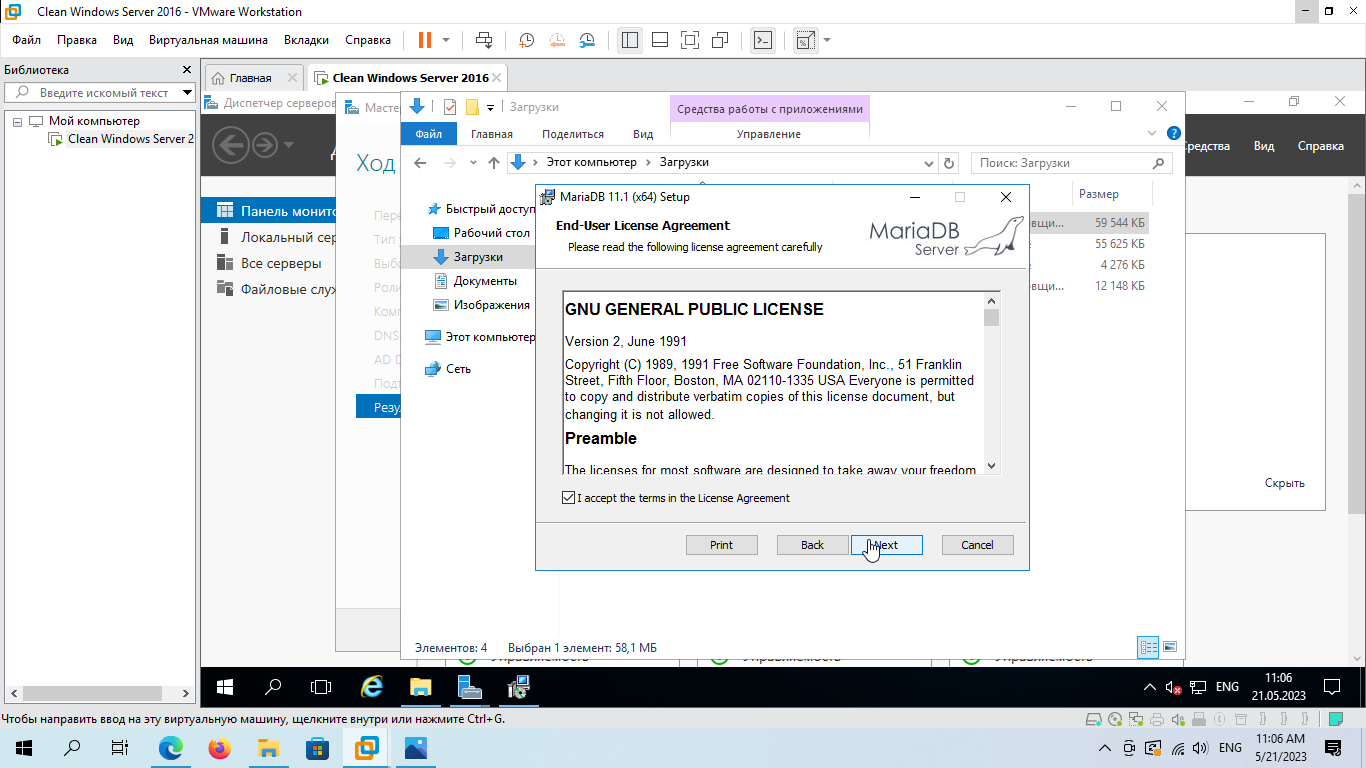
\includegraphics[width=\textwidth]{11_0018}
    \label{img:18}
    \caption{Соглашаемся с условиями использования}
  \end{figure}

  \begin{figure}[H]
    \centering
    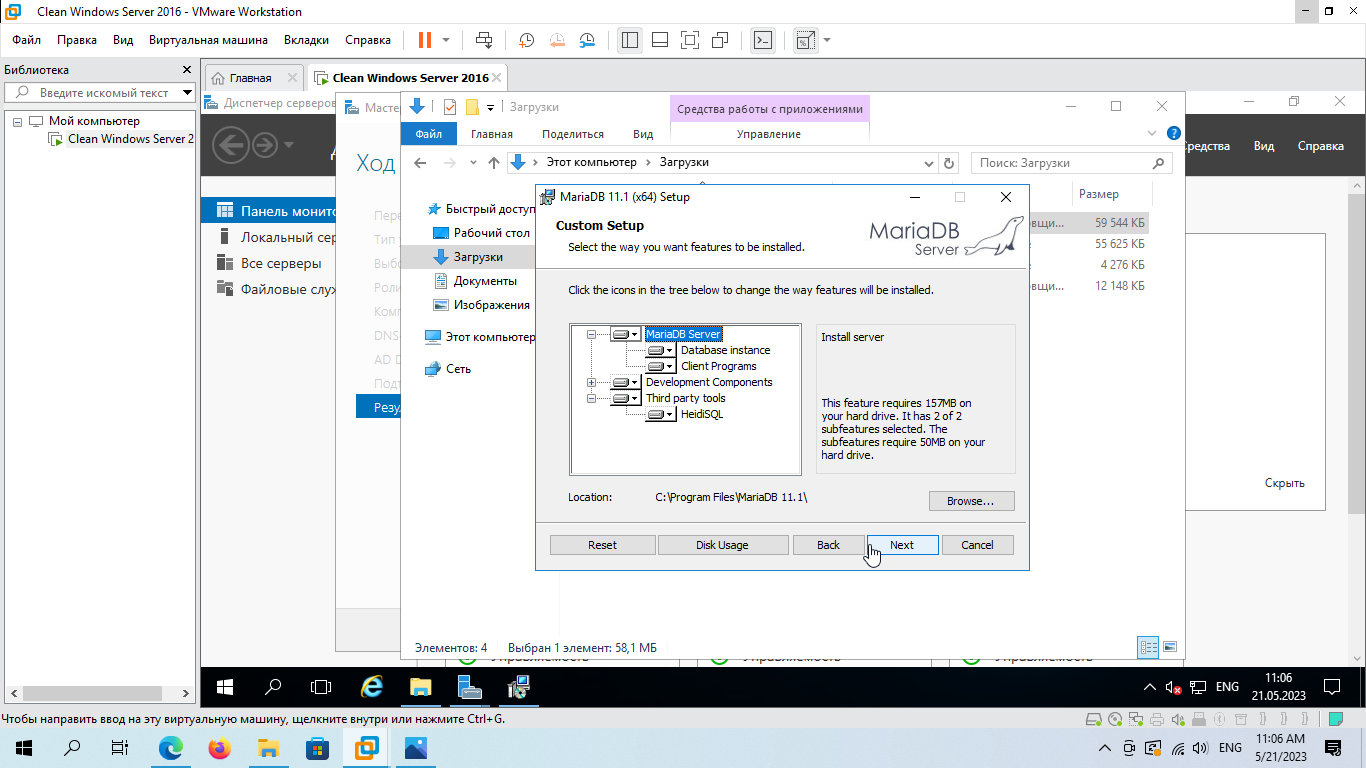
\includegraphics[width=\textwidth]{11_0019}
    \label{img:19}
    \caption{Устанавливаем все возможные компоненты}
  \end{figure}

  \begin{figure}[H]
    \centering
    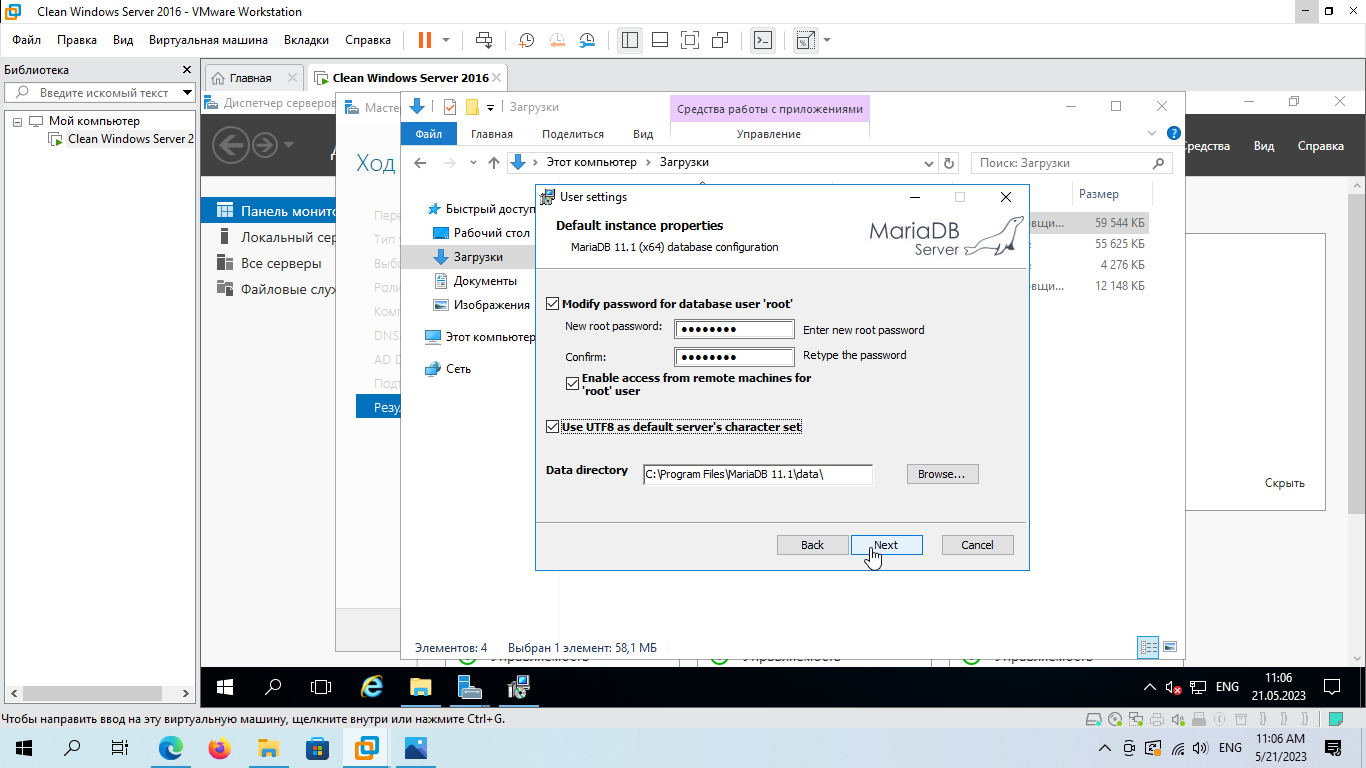
\includegraphics[width=\textwidth]{11_0020}
    \label{img:20}
    \caption{Указываем пароль для пользователя \textit{root}}
  \end{figure}

  \begin{figure}[H]
    \centering
    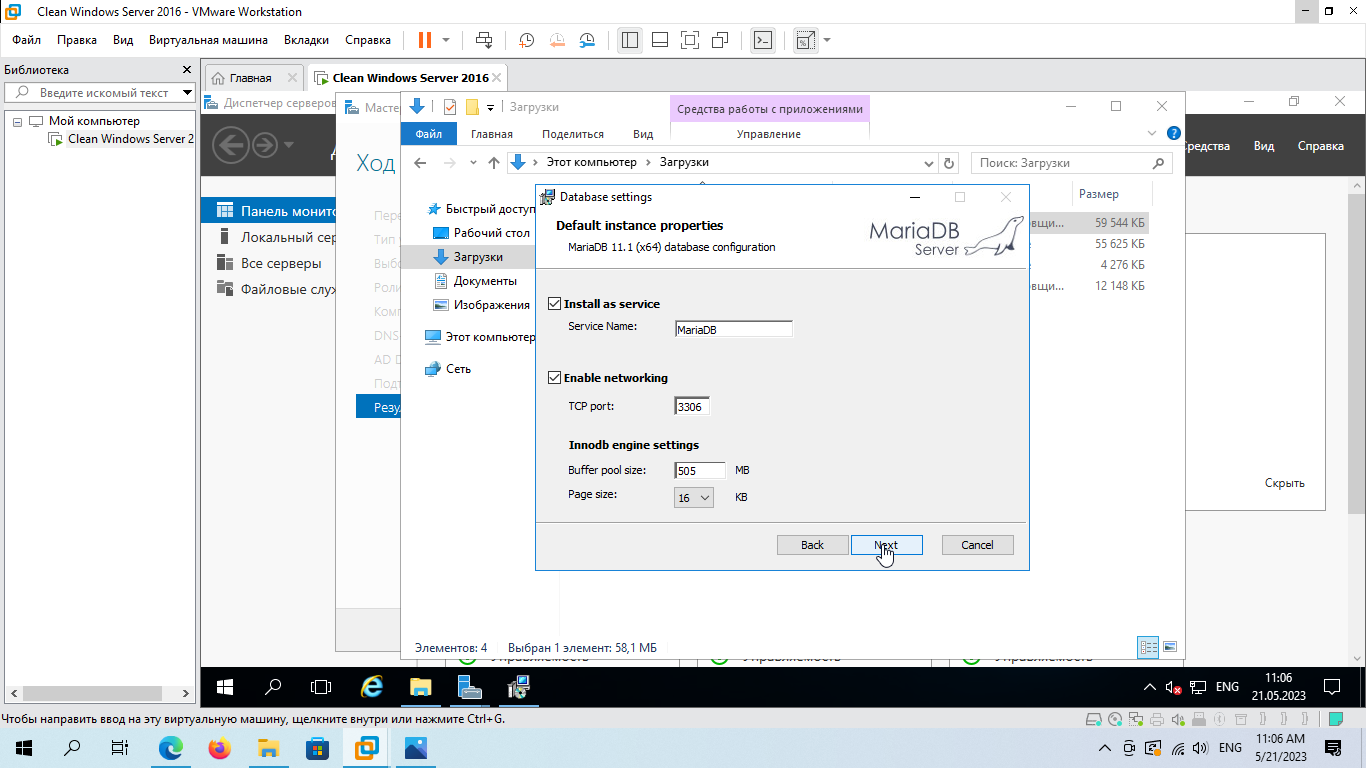
\includegraphics[width=\textwidth]{11_0021}
    \label{img:21}
    \caption{Порт для подключения оставляем по умолчанию}
  \end{figure}

  \begin{figure}[H]
    \centering
    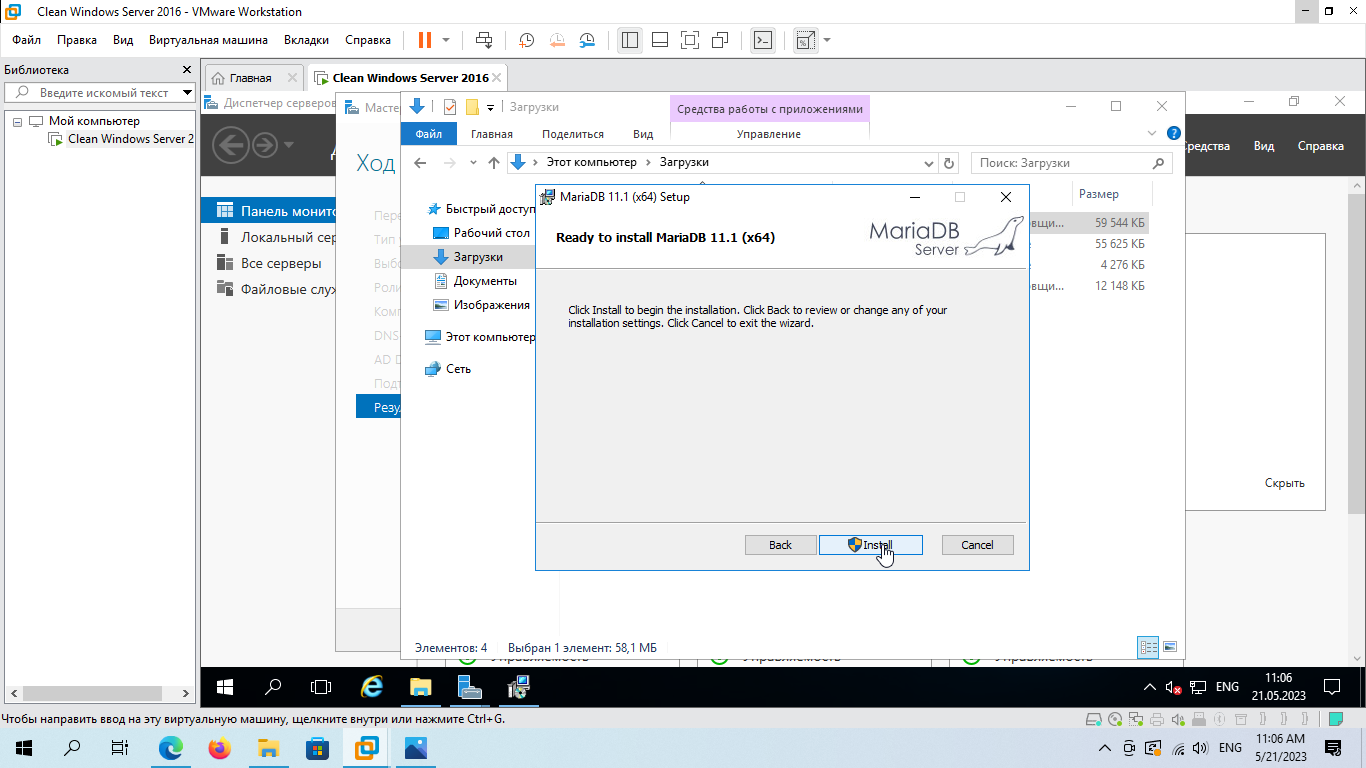
\includegraphics[width=\textwidth]{11_0022}
    \label{img:22}
    \caption{Начинаем установку}
  \end{figure}

  Сама база данных установлена и готова к работе, теперь проинсталлируем
  спецаильный коннектор для данной базы:

  \begin{figure}[H]
    \centering
    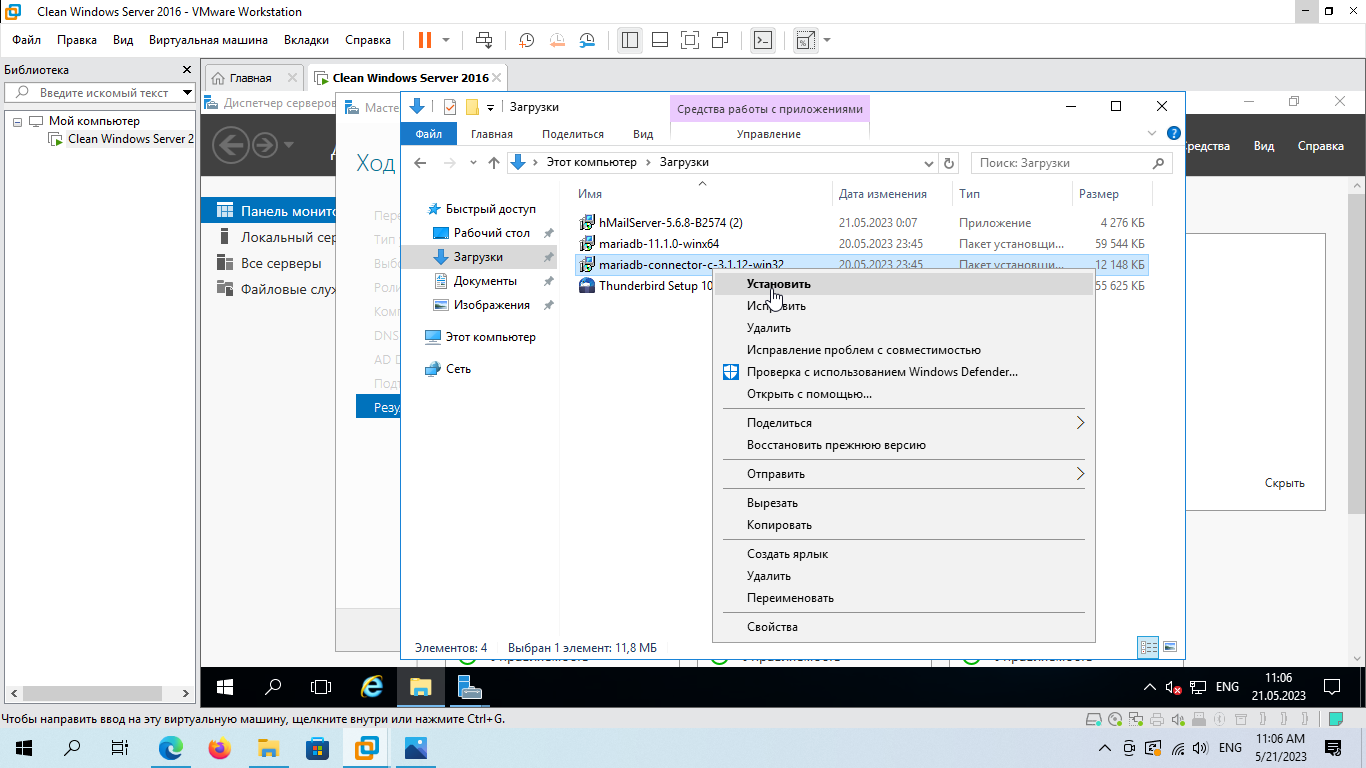
\includegraphics[width=\textwidth]{11_0023}
    \label{img:23}
    \caption{Запускаем установщик}
  \end{figure}

  \begin{figure}[H]
    \centering
    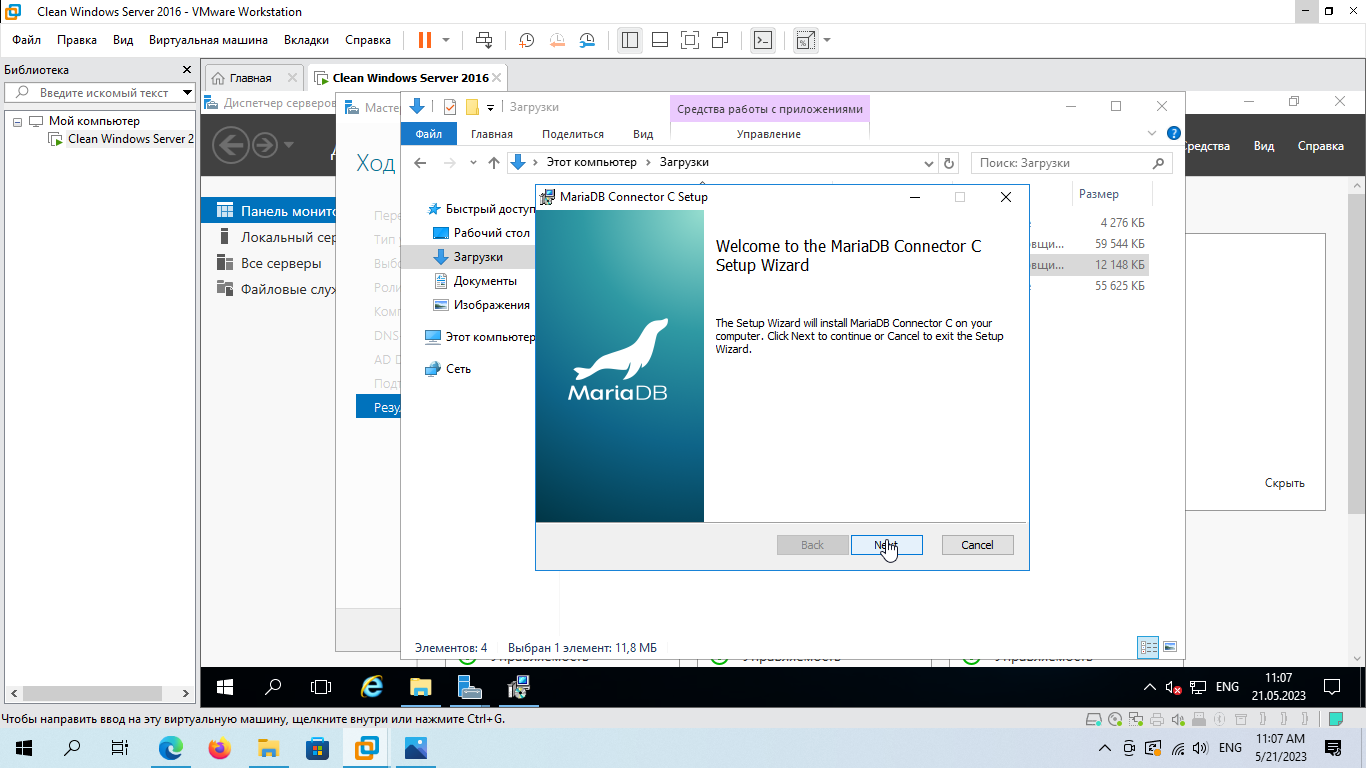
\includegraphics[width=\textwidth]{11_0024}
    \label{img:24}
    \caption{Далее}
  \end{figure}

  \begin{figure}[H]
    \centering
    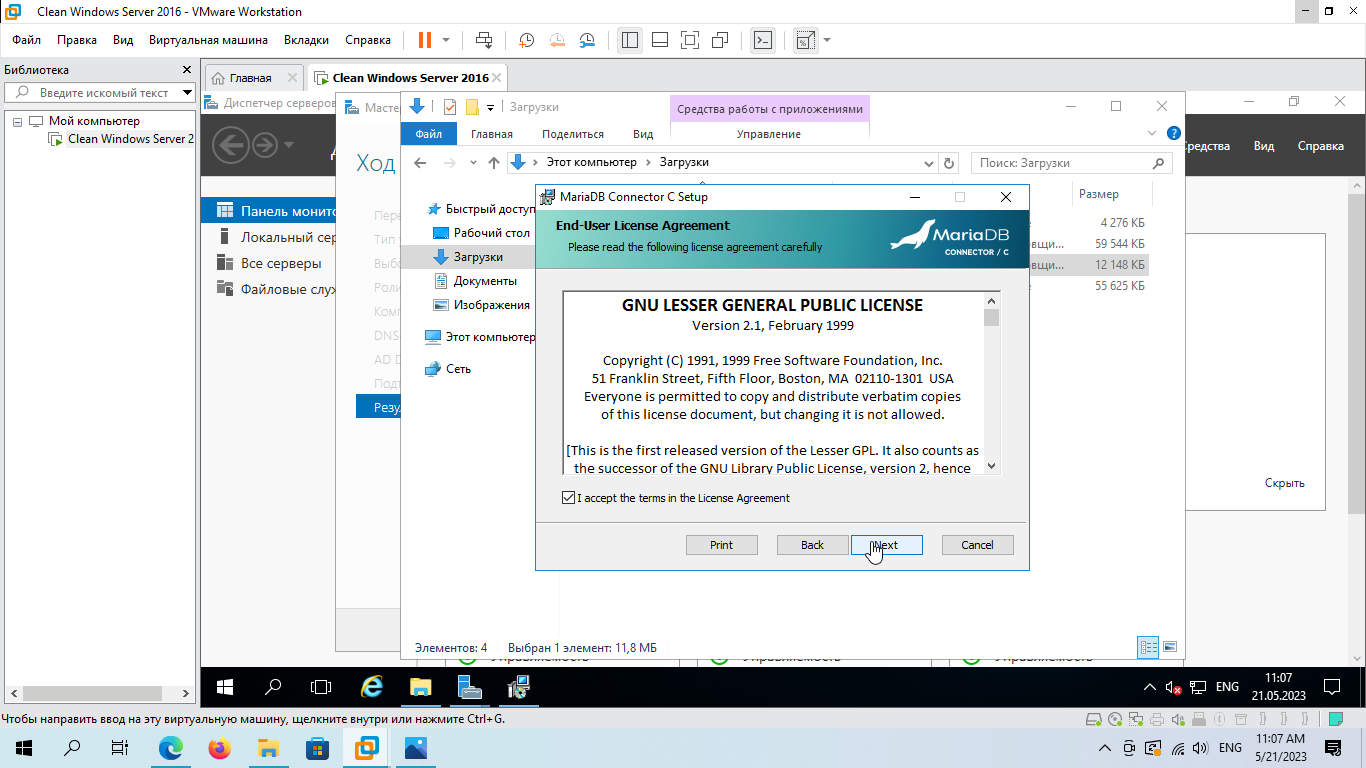
\includegraphics[width=\textwidth]{11_0025}
    \label{img:25}
    \caption{Соглашаемся с условиями использования}
  \end{figure}

  \begin{figure}[H]
    \centering
    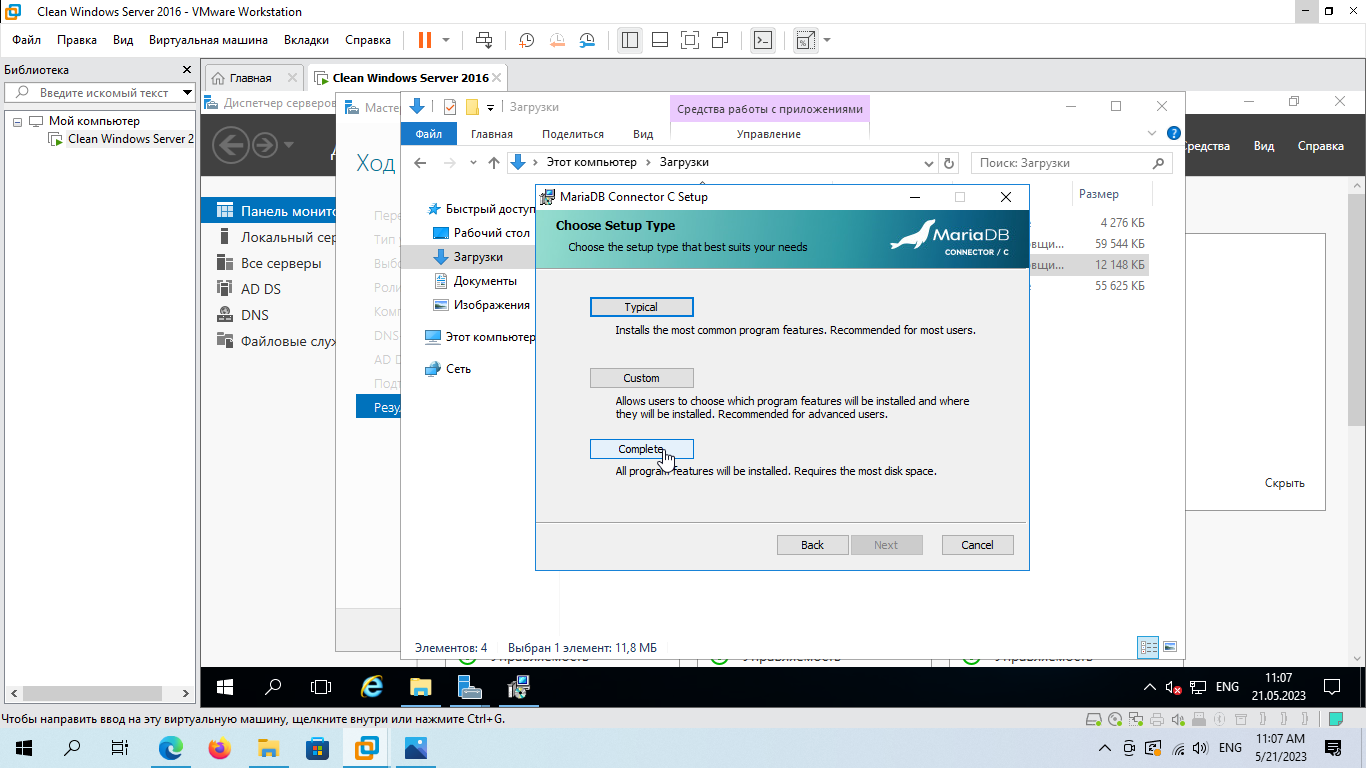
\includegraphics[width=\textwidth]{11_0026}
    \label{img:26}
    \caption{Тип установки - полная}
  \end{figure}

  \begin{figure}[H]
    \centering
    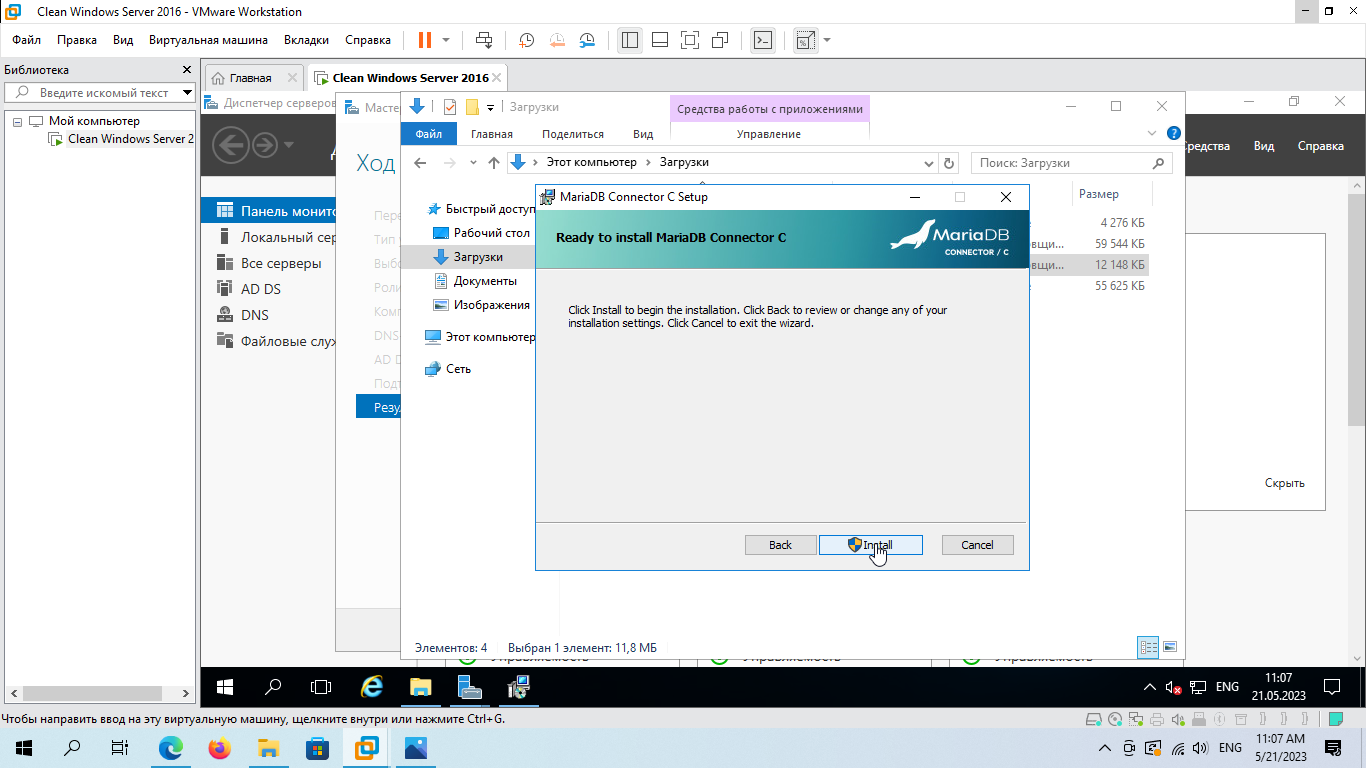
\includegraphics[width=\textwidth]{11_0027}
    \label{img:27}
    \caption{Установить}
  \end{figure}

  \begin{figure}[H]
    \centering
    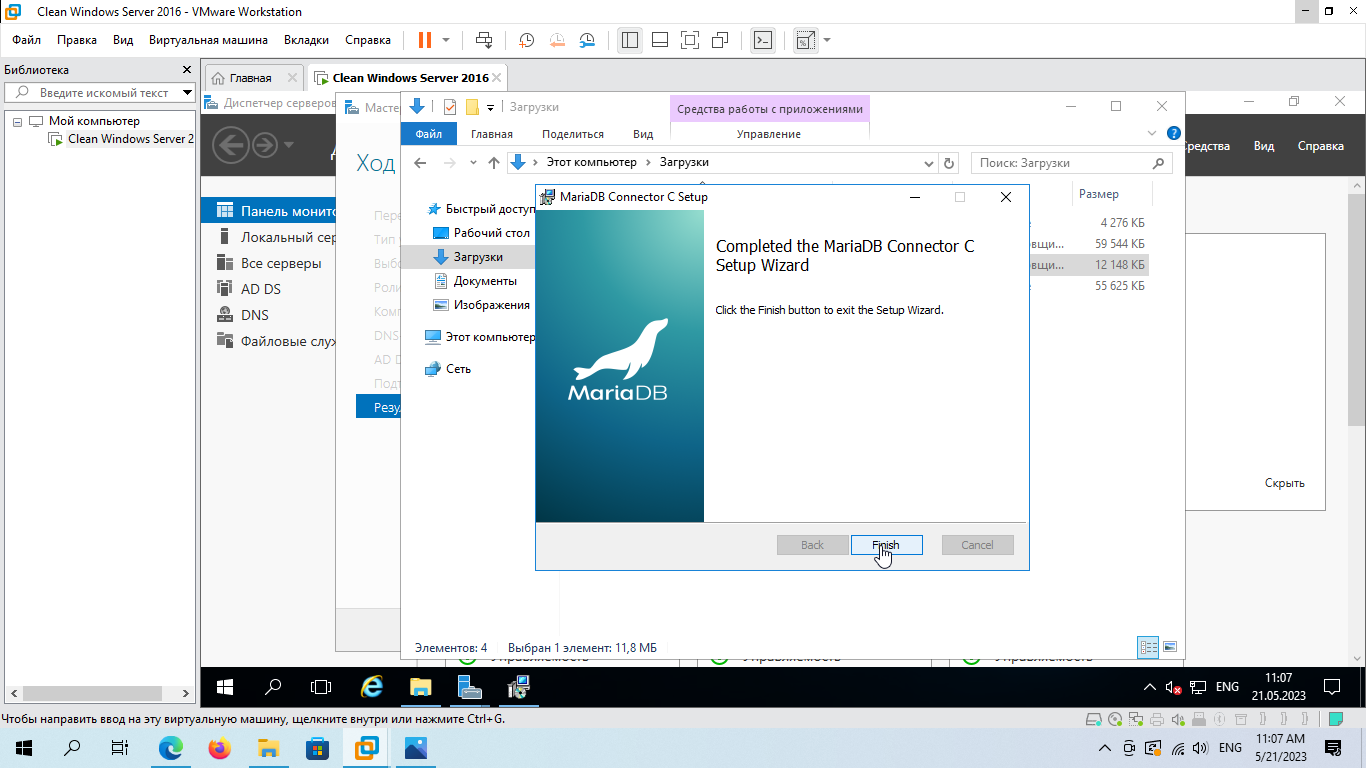
\includegraphics[width=\textwidth]{11_0028}
    \label{img:28}
    \caption{Установка завершена}
  \end{figure}

  Для проверки настроенного почтового сервера потребуется почтовый клиент - установим его:

  \begin{figure}[H]
    \centering
    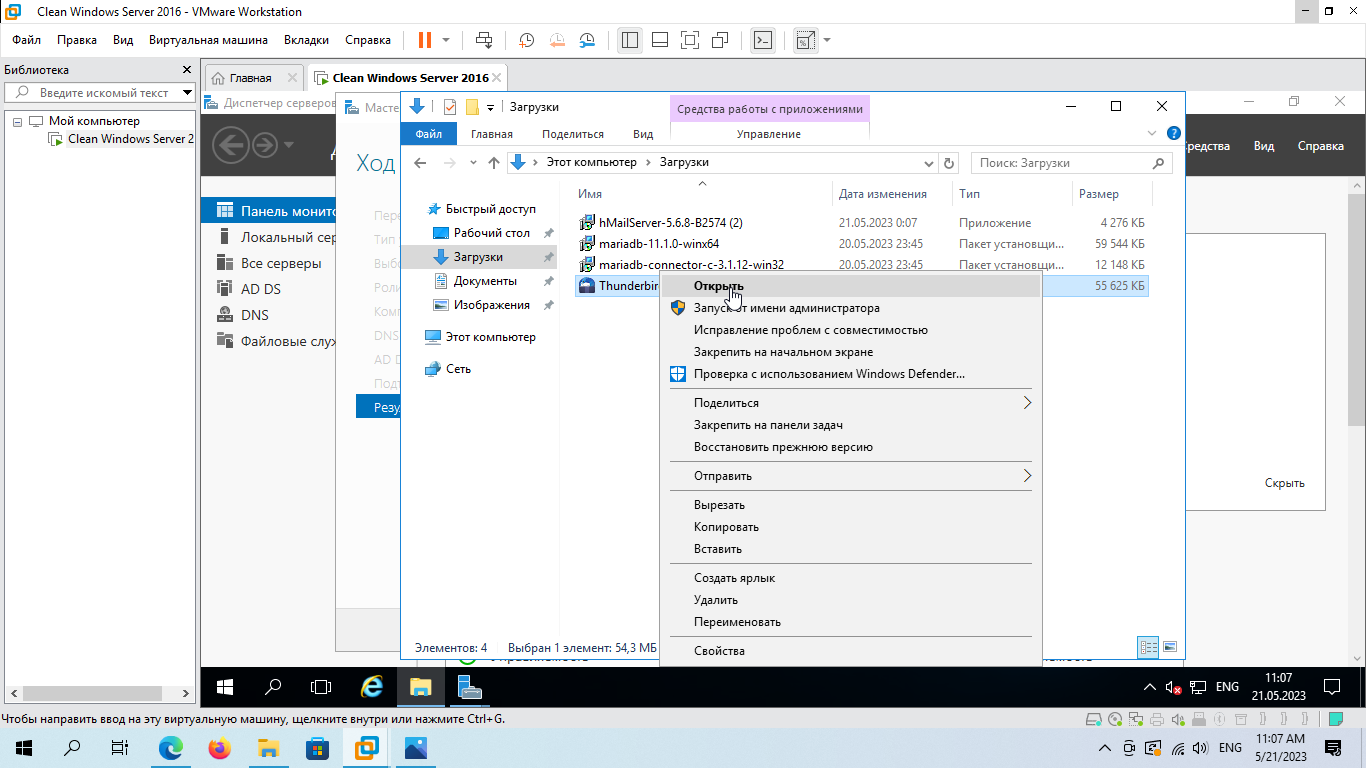
\includegraphics[width=\textwidth]{11_0029}
    \label{img:29}
    \caption{Запускаем установку \textit{Thunderbird}}
  \end{figure}

  \begin{figure}[H]
    \centering
    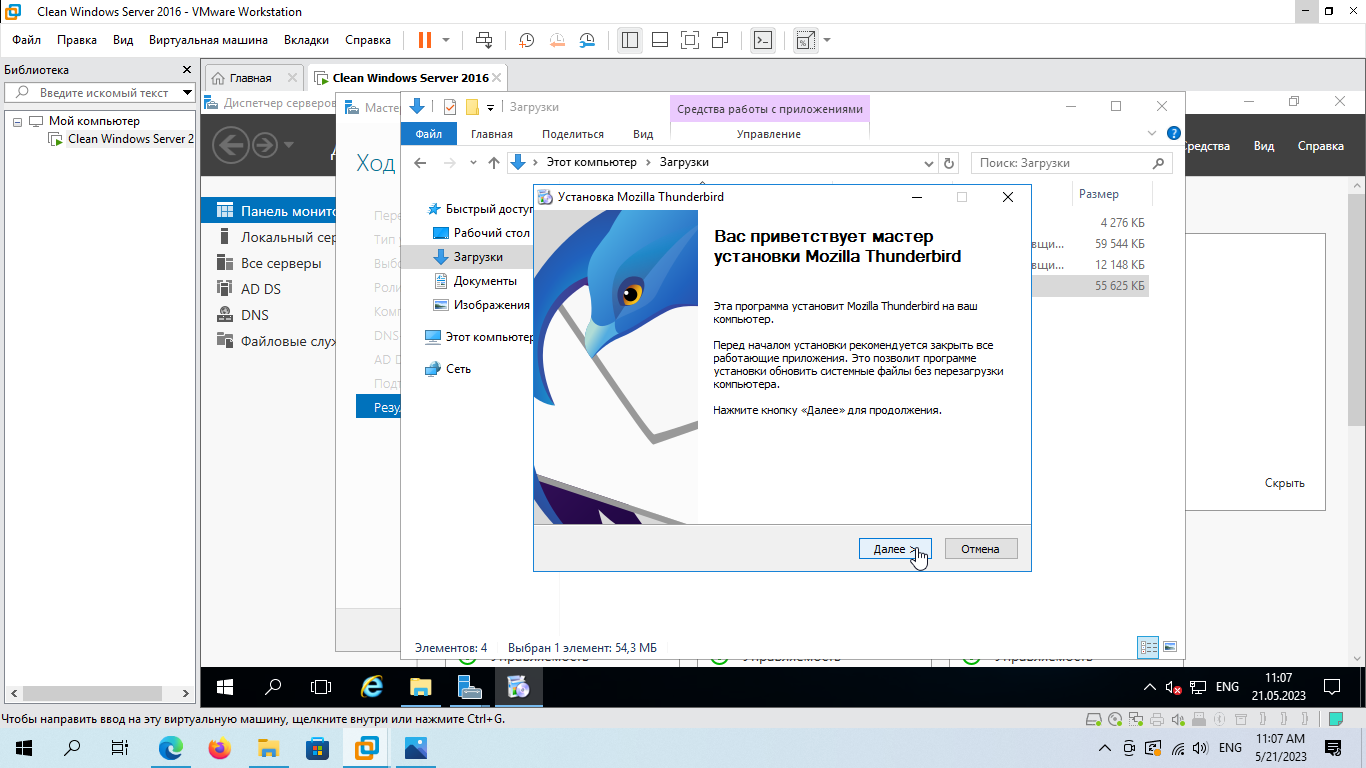
\includegraphics[width=\textwidth]{11_0030}
    \label{img:30}
    \caption{Далее}
  \end{figure}

  \begin{figure}[H]
    \centering
    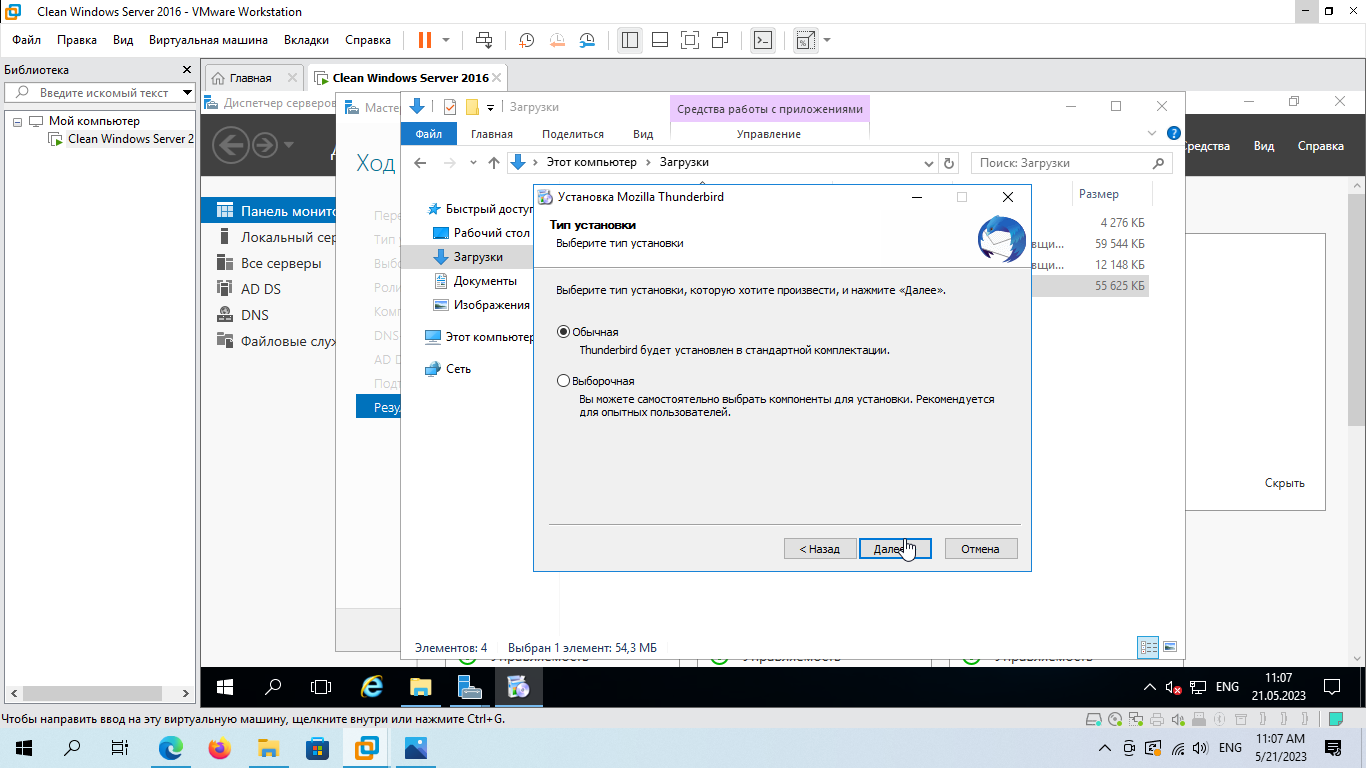
\includegraphics[width=\textwidth]{11_0031}
    \label{img:31}
    \caption{Обычная установка - все компоненты}
  \end{figure}

  \begin{figure}[H]
    \centering
    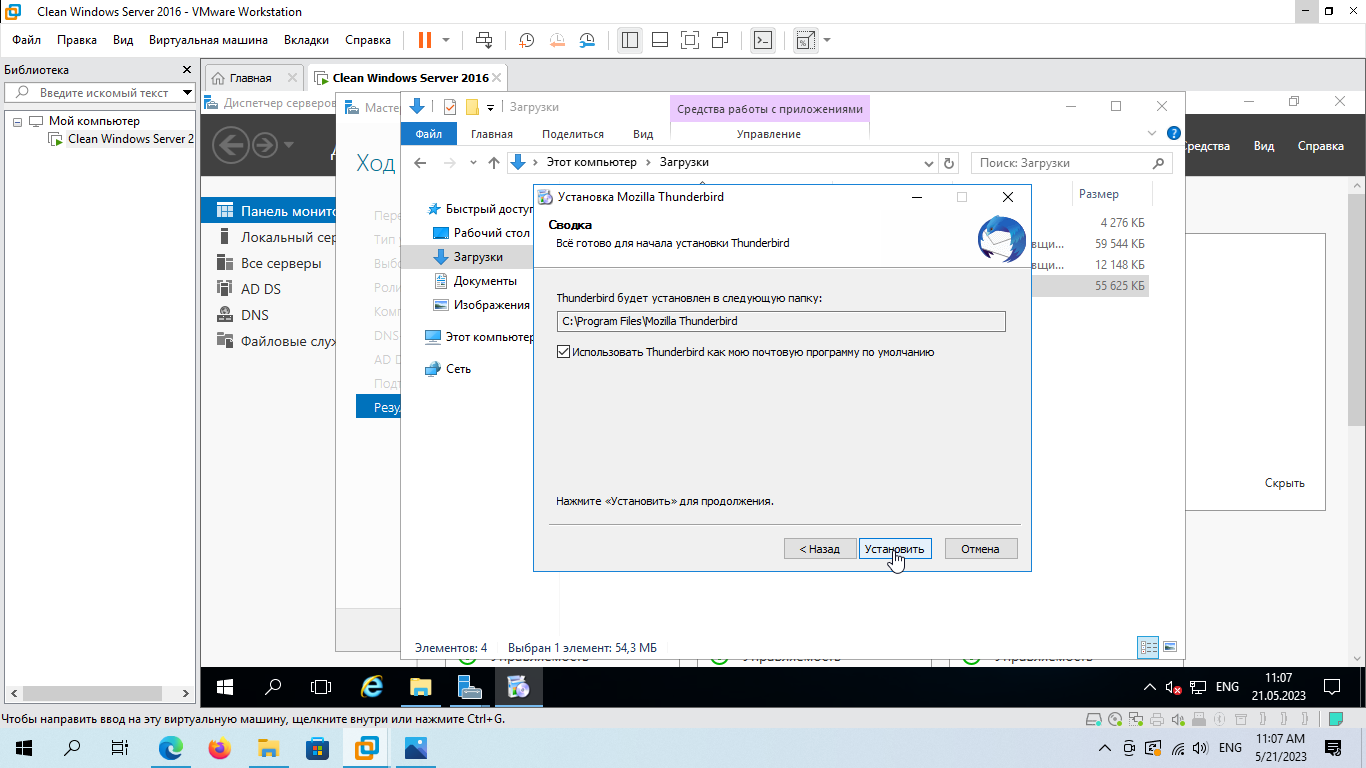
\includegraphics[width=\textwidth]{11_0032}
    \label{img:32}
    \caption{Далее}
  \end{figure}

  \begin{figure}[H]
    \centering
    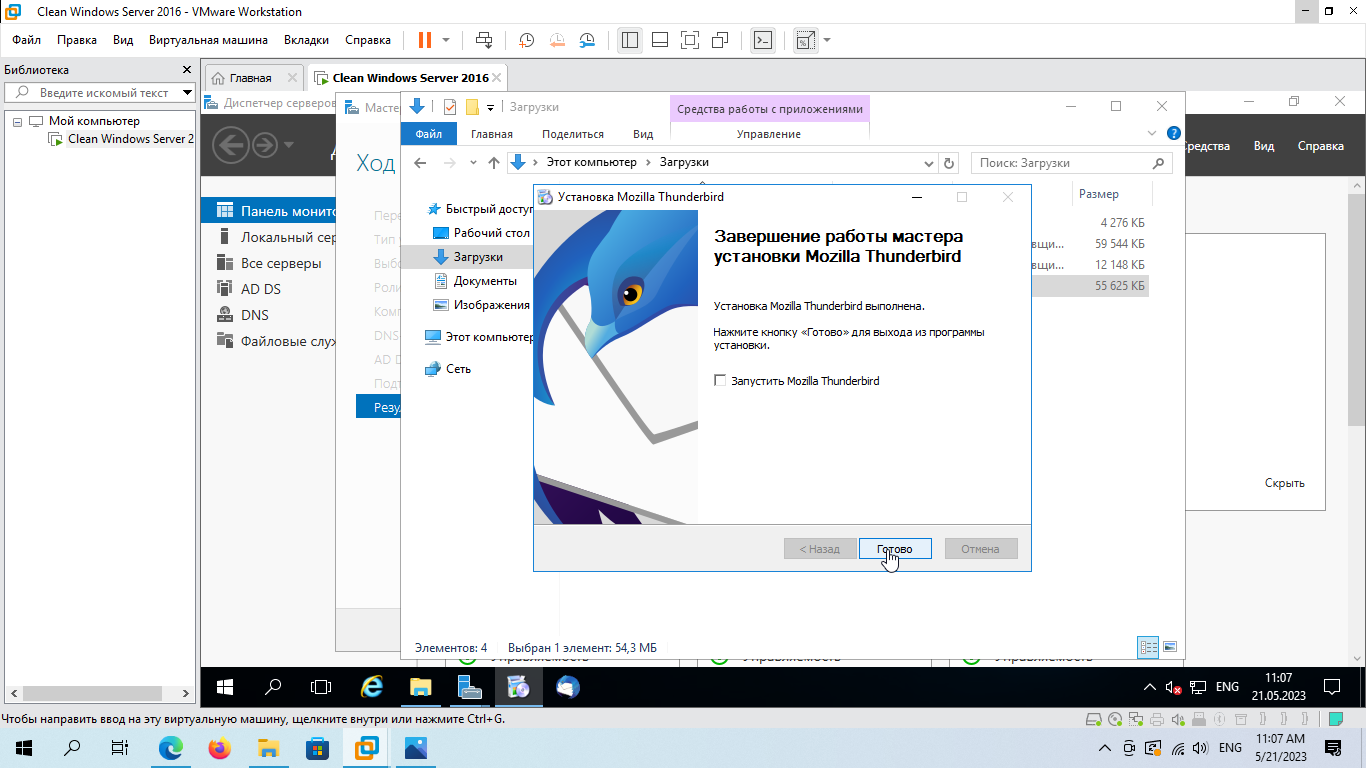
\includegraphics[width=\textwidth]{11_0033}
    \label{img:33}
    \caption{Установка завершена}
  \end{figure}

  \begin{figure}[H]
    \centering
    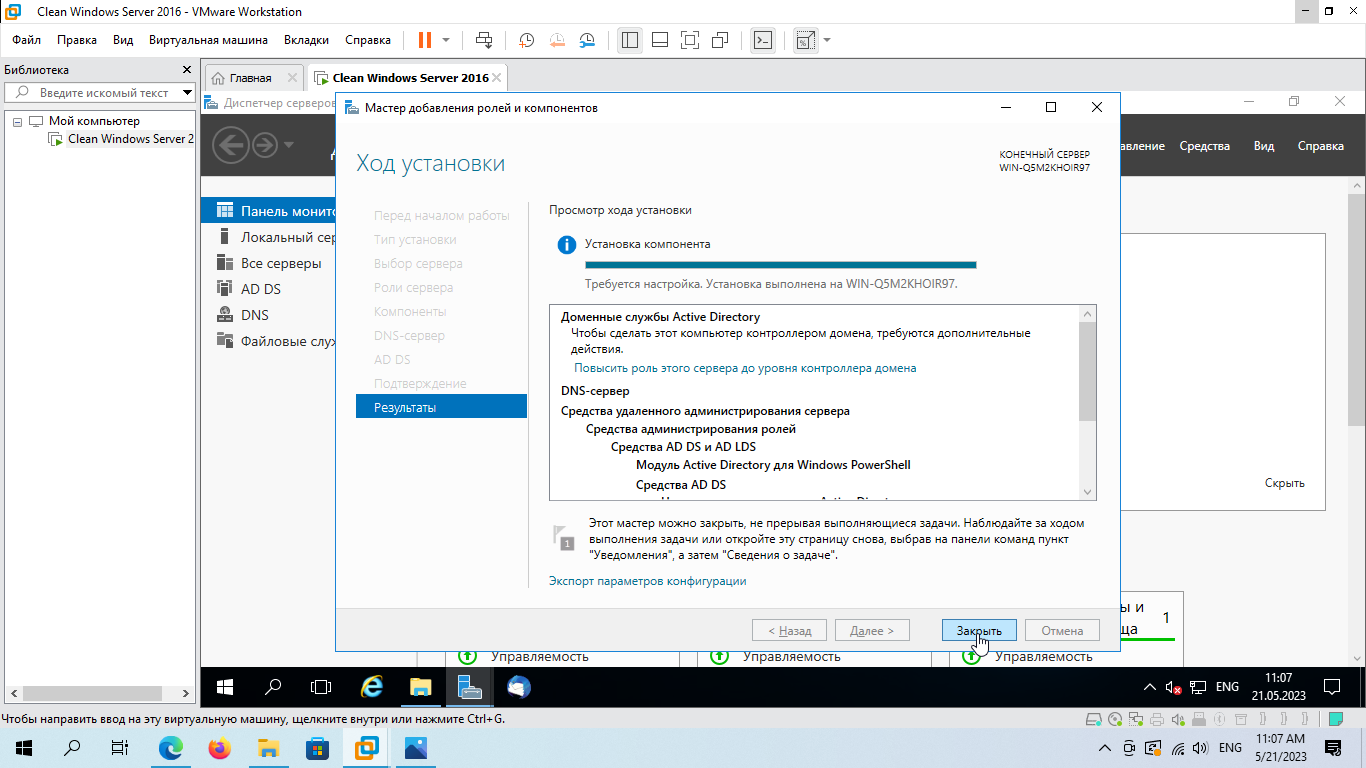
\includegraphics[width=\textwidth]{11_0034}
    \label{img:34}
    \caption{Также завершена и установка системных компонентов}
  \end{figure}

  \subsection{Настройка домена}

  \begin{figure}[H]
    \centering
    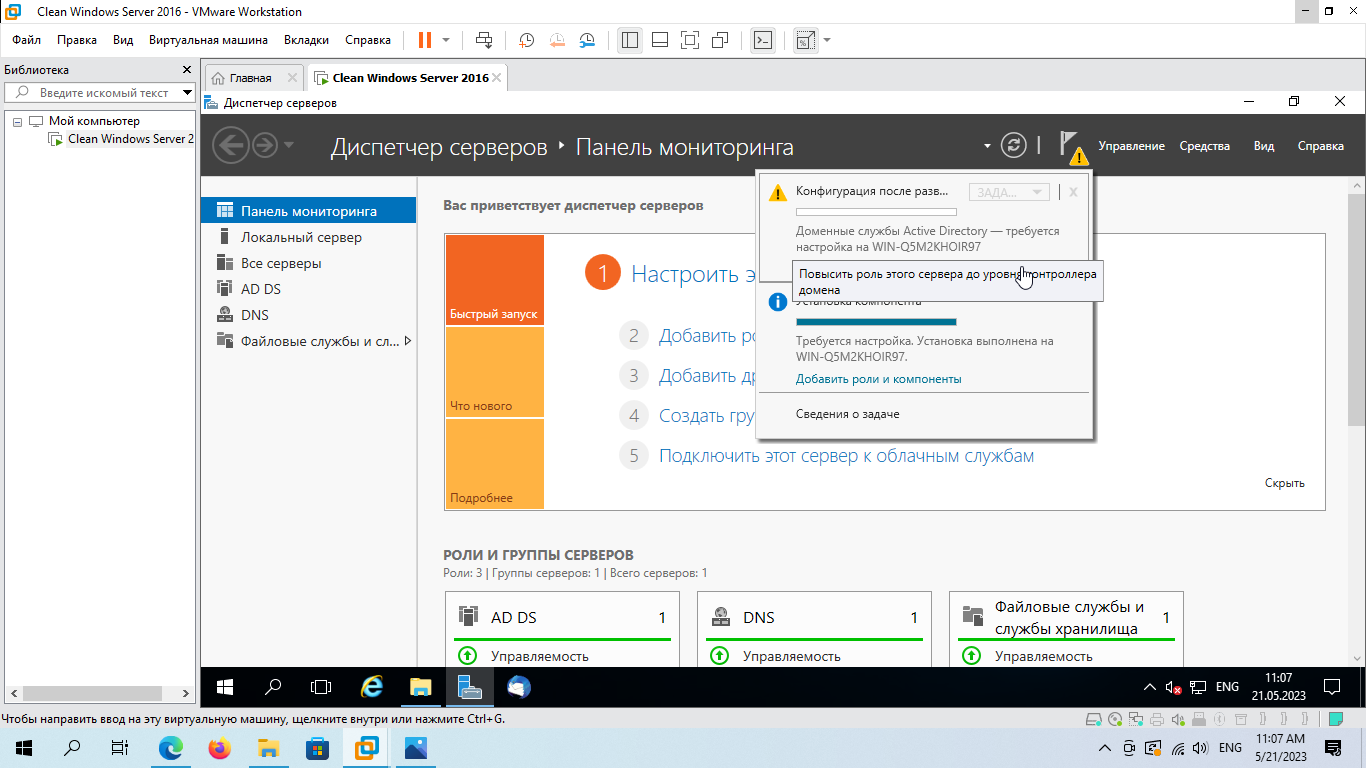
\includegraphics[width=\textwidth]{11_0035}
    \label{img:35}
    \caption{Начинаем повышение роли сервера до контроллера домена}
  \end{figure}

  \begin{figure}[H]
    \centering
    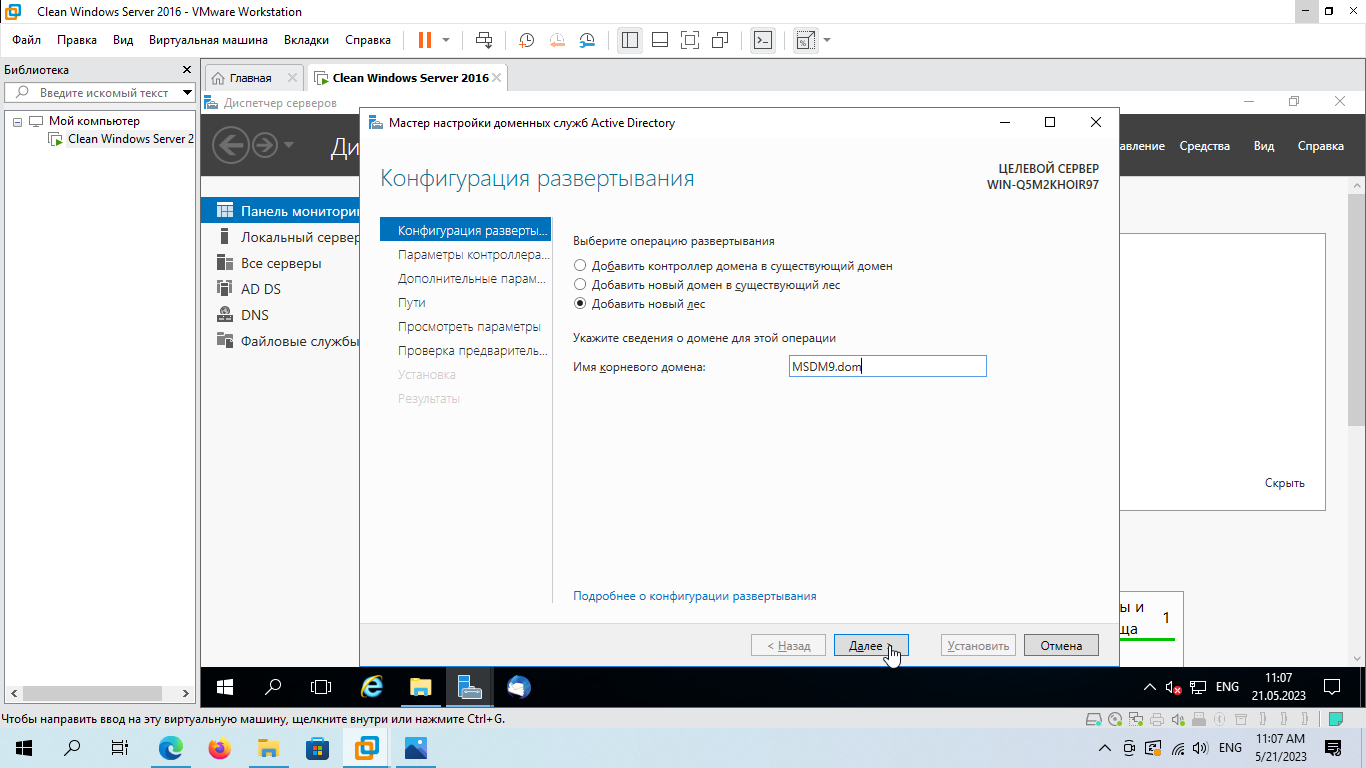
\includegraphics[width=\textwidth]{11_0036}
    \label{img:36}
    \caption{Вводим имя домена}
  \end{figure}

  \begin{figure}[H]
    \centering
    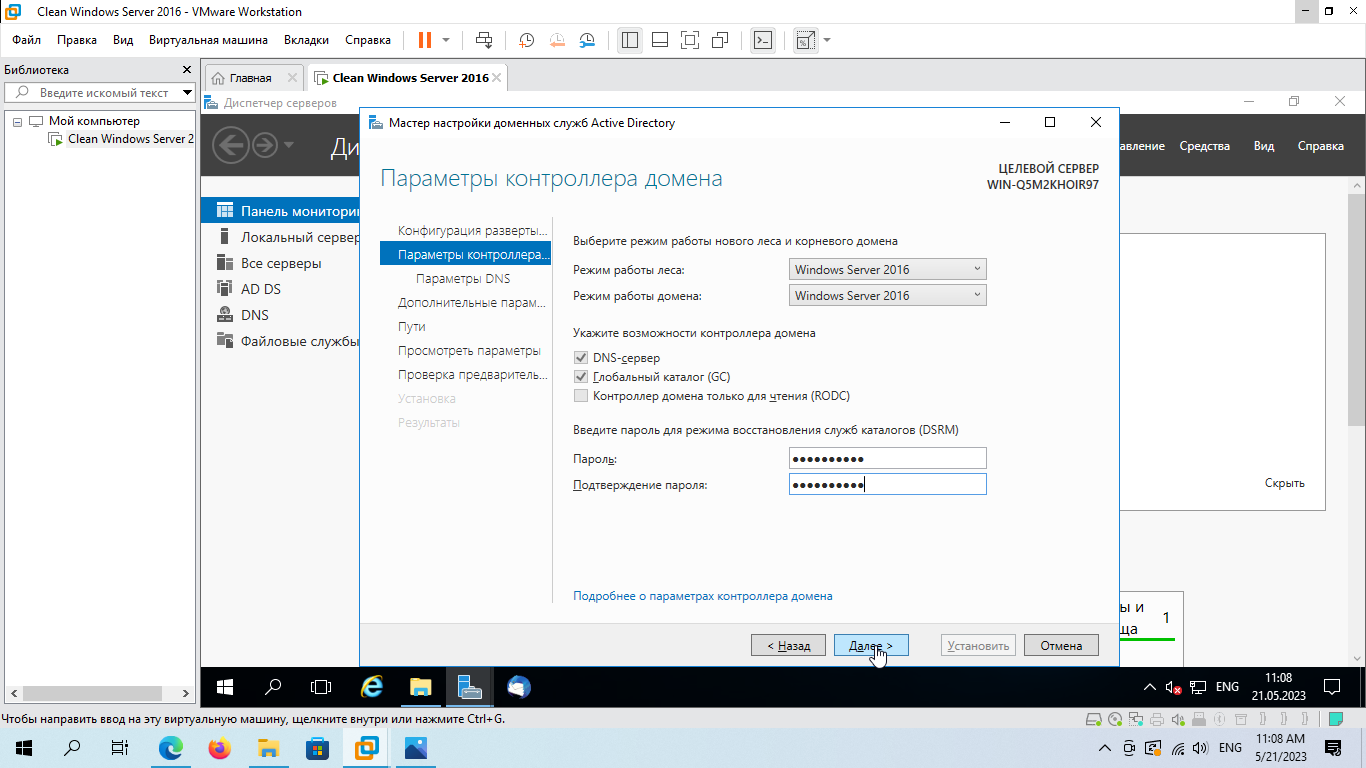
\includegraphics[width=\textwidth]{11_0037}
    \label{img:37}
    \caption{Устанваливаем пароь для режима восстановления}
  \end{figure}

  \begin{figure}[H]
    \centering
    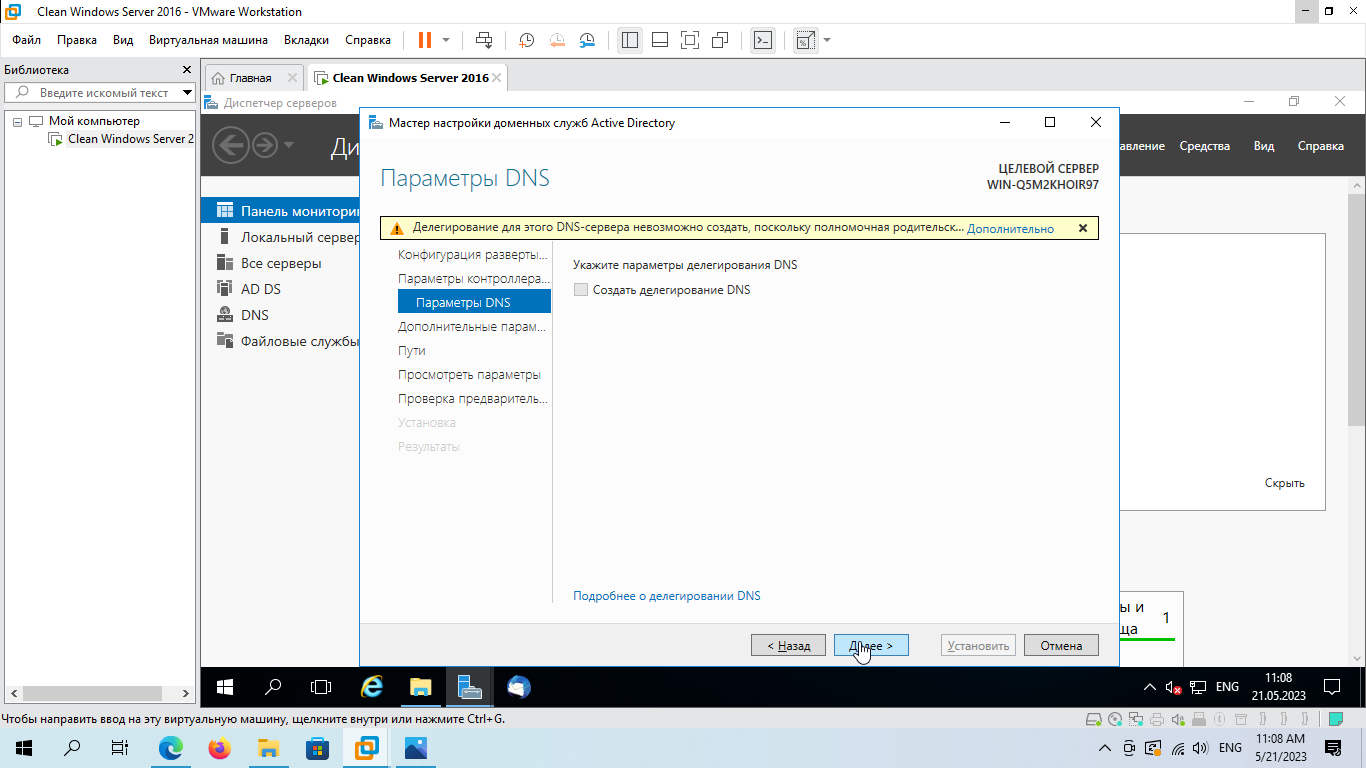
\includegraphics[width=\textwidth]{11_0038}
    \label{img:38}
    \caption{Настройка делегирования DNS невозможна - далее}
  \end{figure}

  \begin{figure}[H]
    \centering
    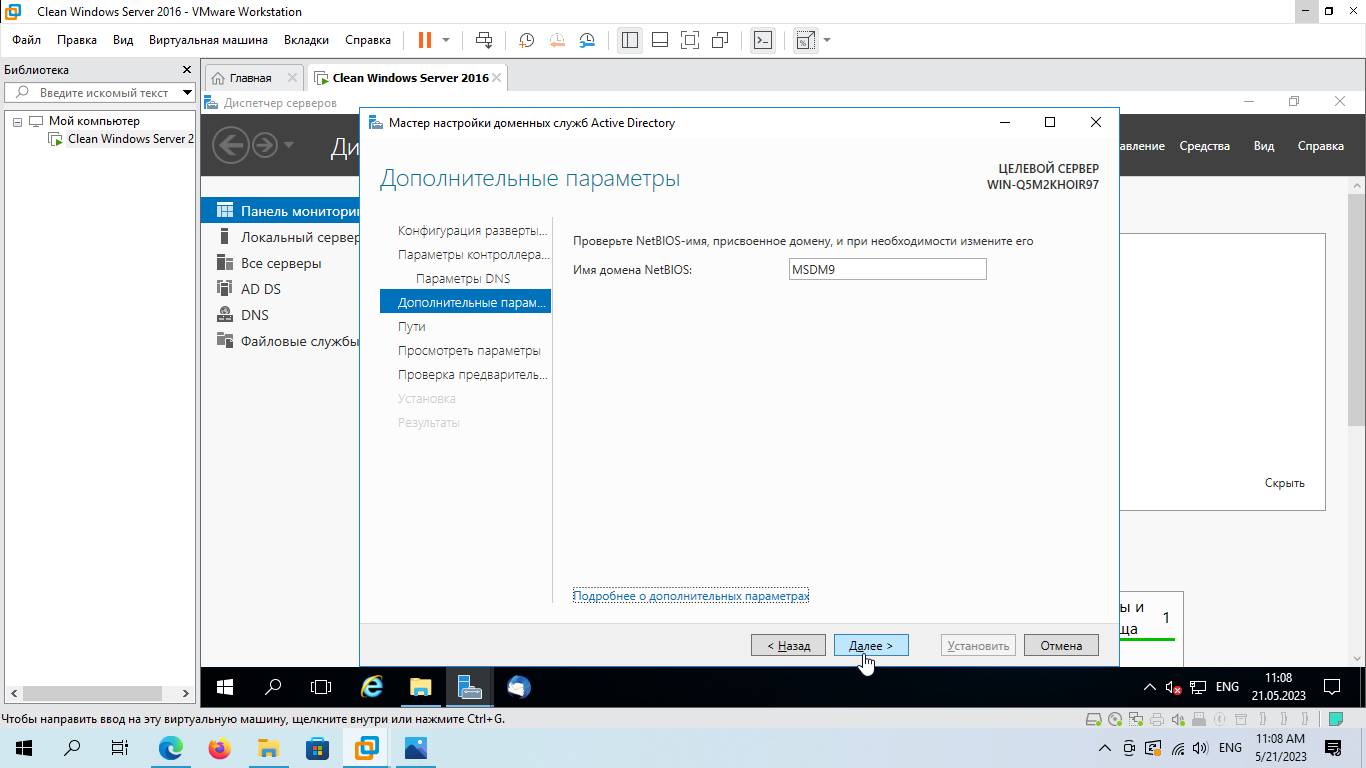
\includegraphics[width=\textwidth]{11_0039}
    \label{img:39}
    \caption{Имя NetBIOS установлено автоматически}
  \end{figure}

  \begin{figure}[H]
    \centering
    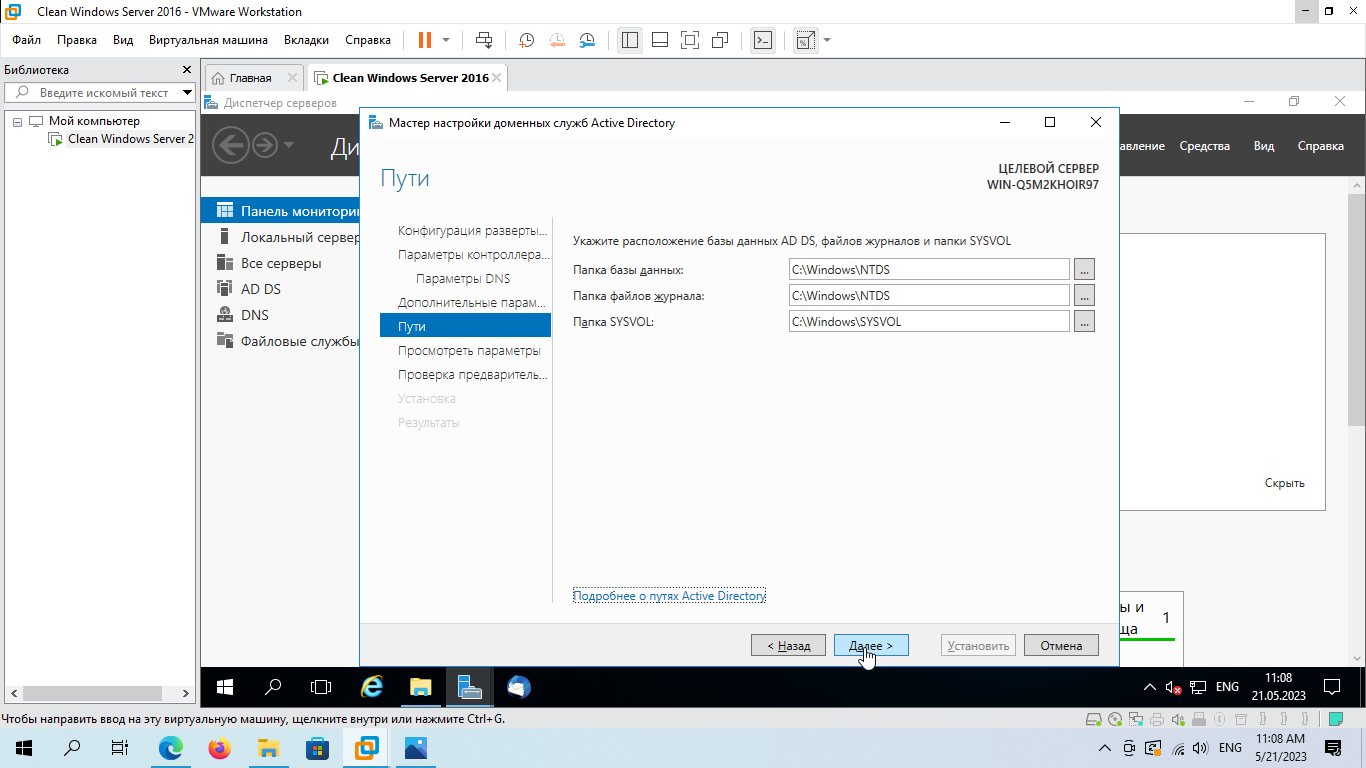
\includegraphics[width=\textwidth]{11_0040}
    \label{img:40}
    \caption{Далее}
  \end{figure}

  \begin{figure}[H]
    \centering
    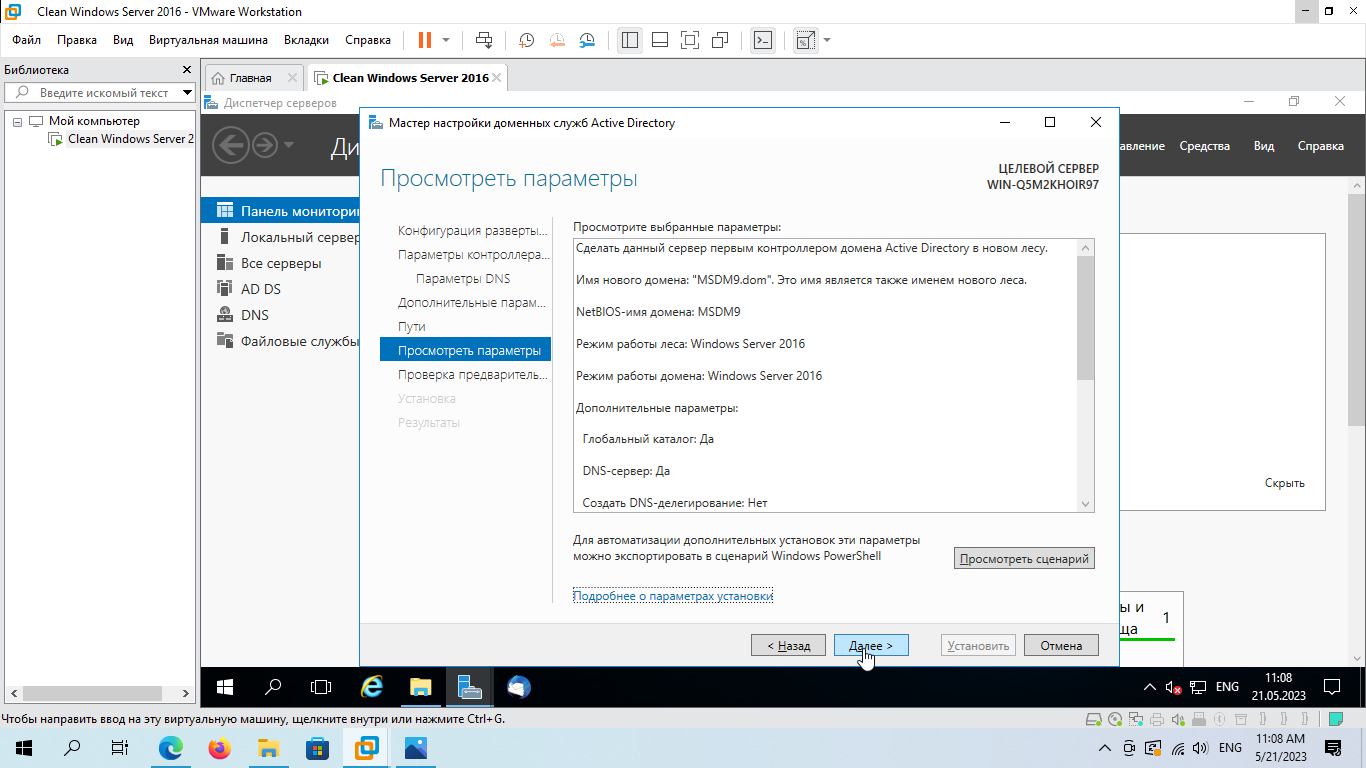
\includegraphics[width=\textwidth]{11_0041}
    \label{img:41}
    \caption{Далее}
  \end{figure}

  \begin{figure}[H]
    \centering
    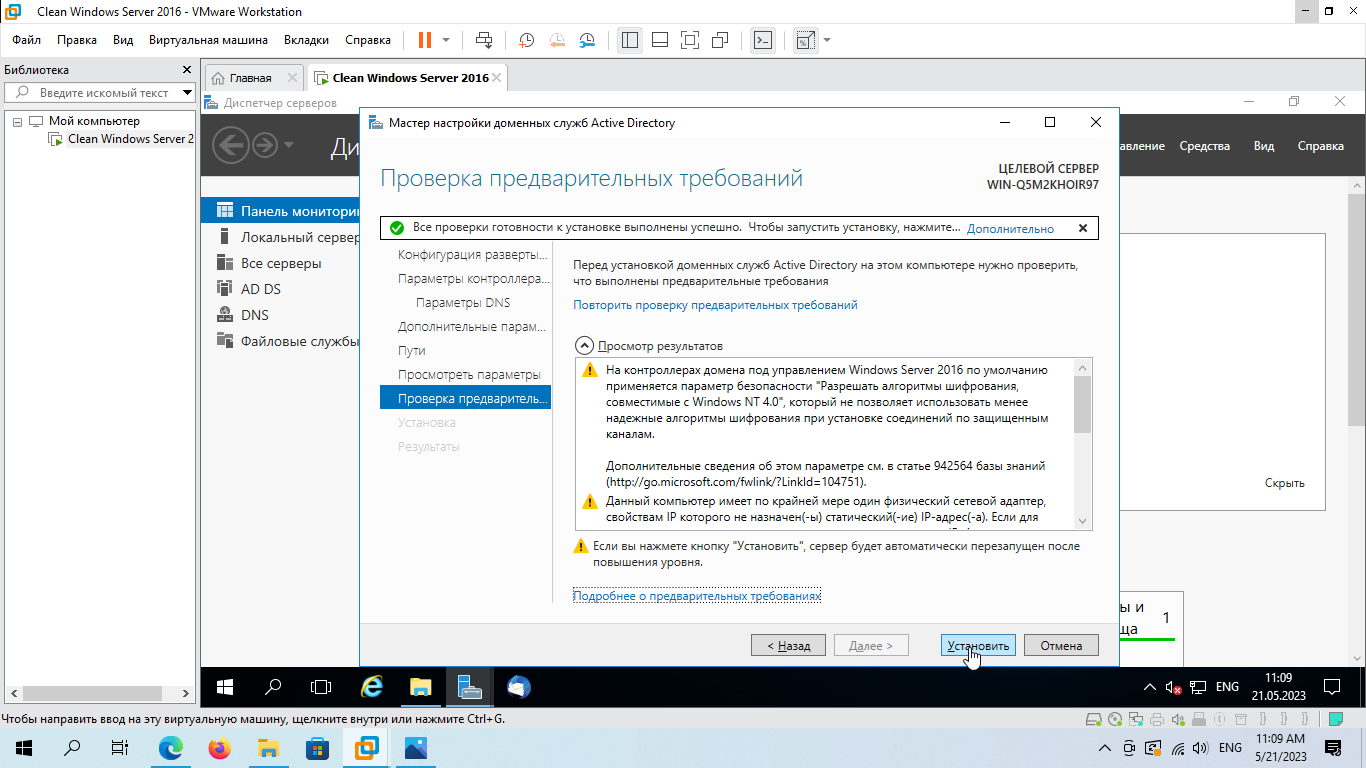
\includegraphics[width=\textwidth]{11_0042}
    \label{img:42}
    \caption{Начинаем установку - повышение роли}
  \end{figure}

  \begin{figure}[H]
    \centering
    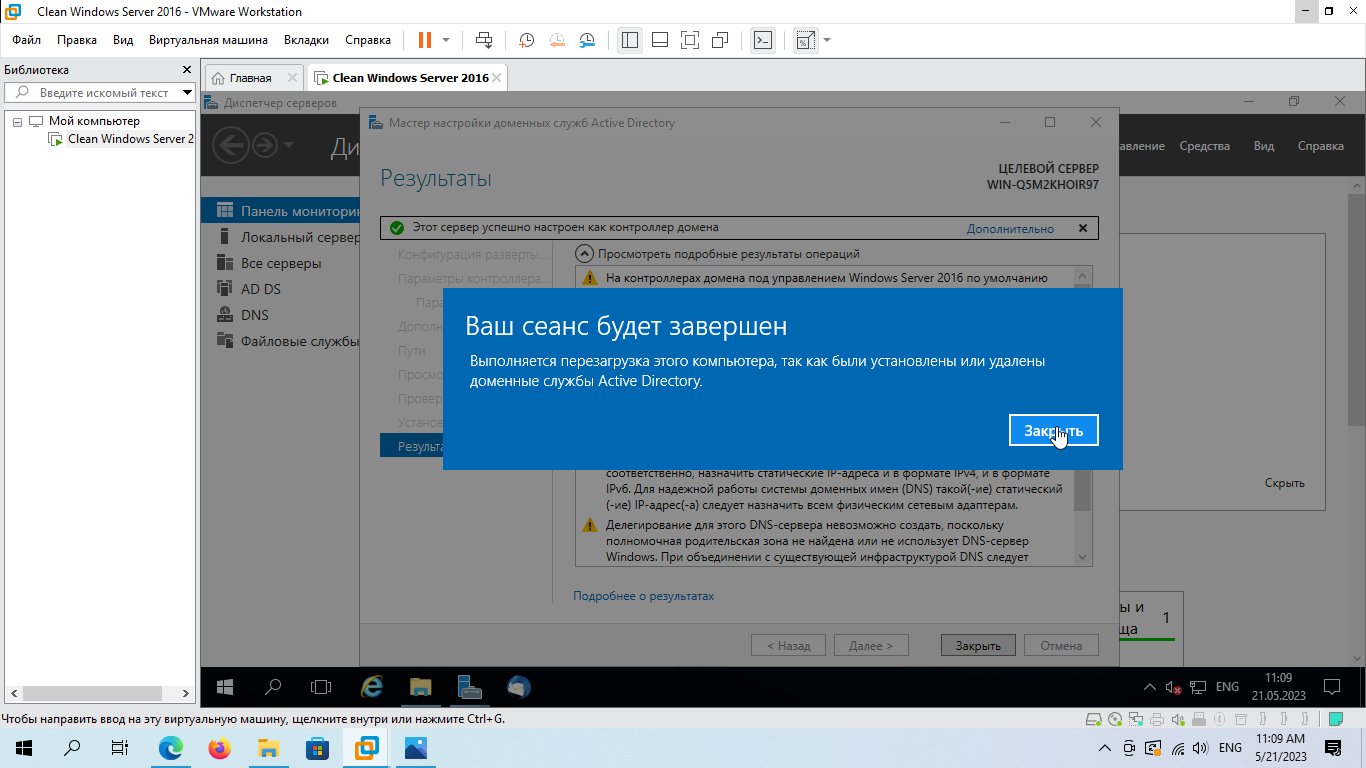
\includegraphics[width=\textwidth]{11_0043}
    \label{img:43}
    \caption{Необходима перезагрузка}
  \end{figure}

  \begin{figure}[H]
    \centering
    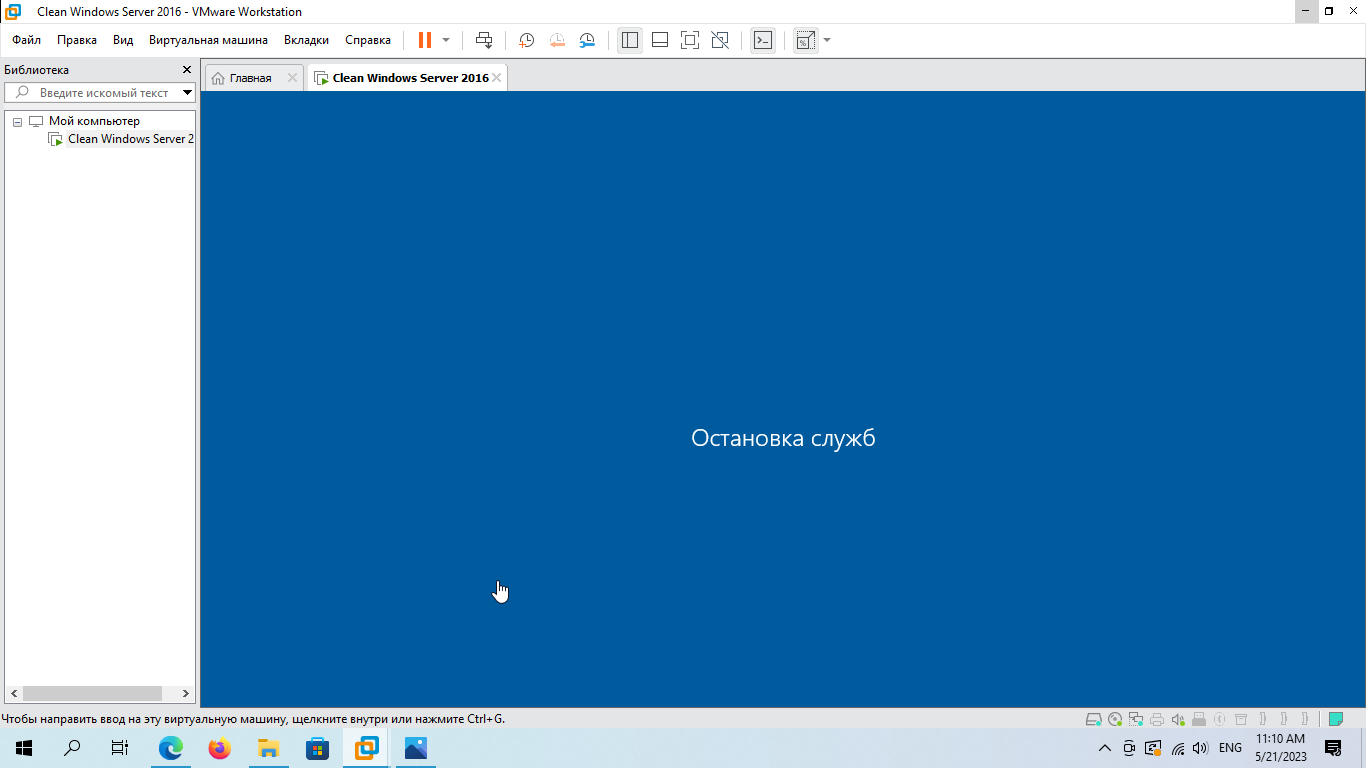
\includegraphics[width=\textwidth]{11_0044}
    \label{img:44}
    \caption{Перезагрузка}
  \end{figure}

  \begin{figure}[H]
    \centering
    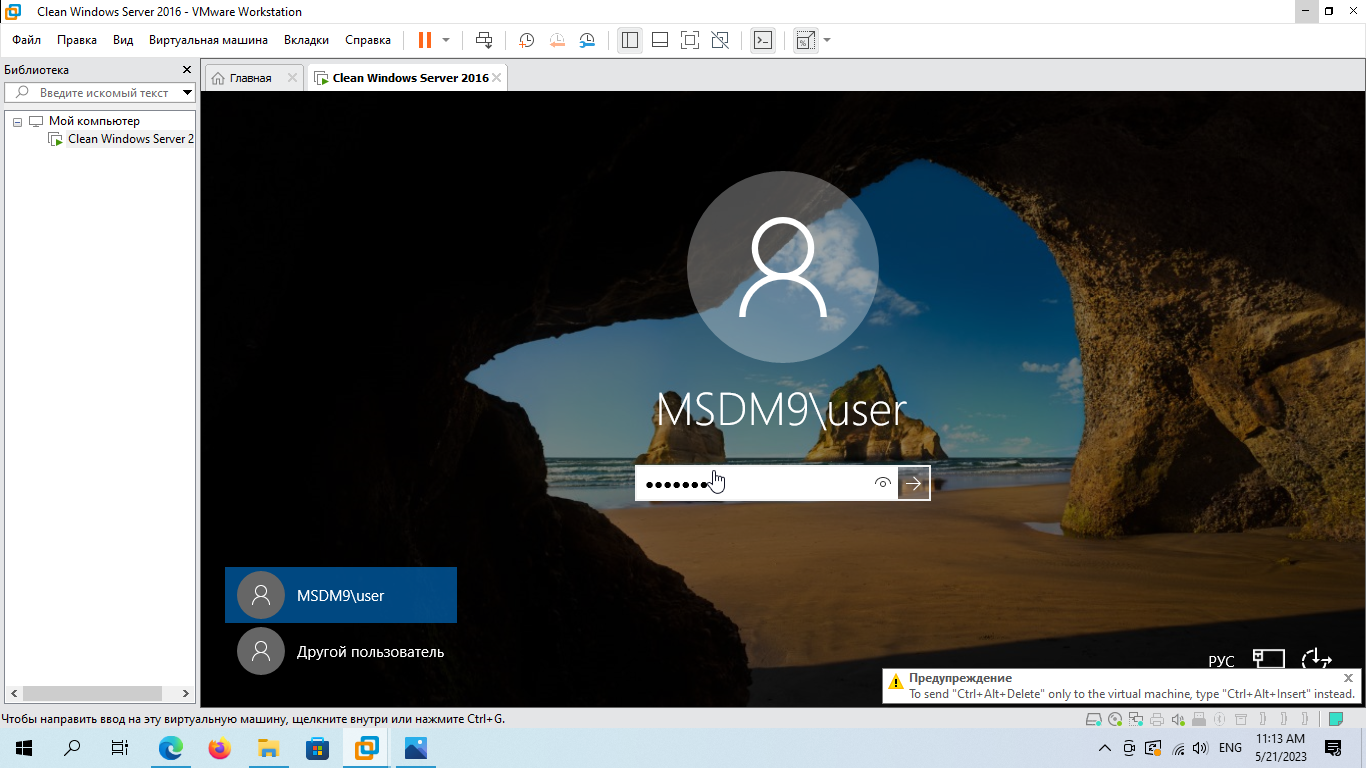
\includegraphics[width=\textwidth]{11_0045}
    \label{img:45}
    \caption{Входим в учетную запись пользователя}
  \end{figure}

  Теперь домен настроен и готов к работе.

  \subsection{Установка и настройка почтового сервера}

  \begin{figure}[H]
    \centering
    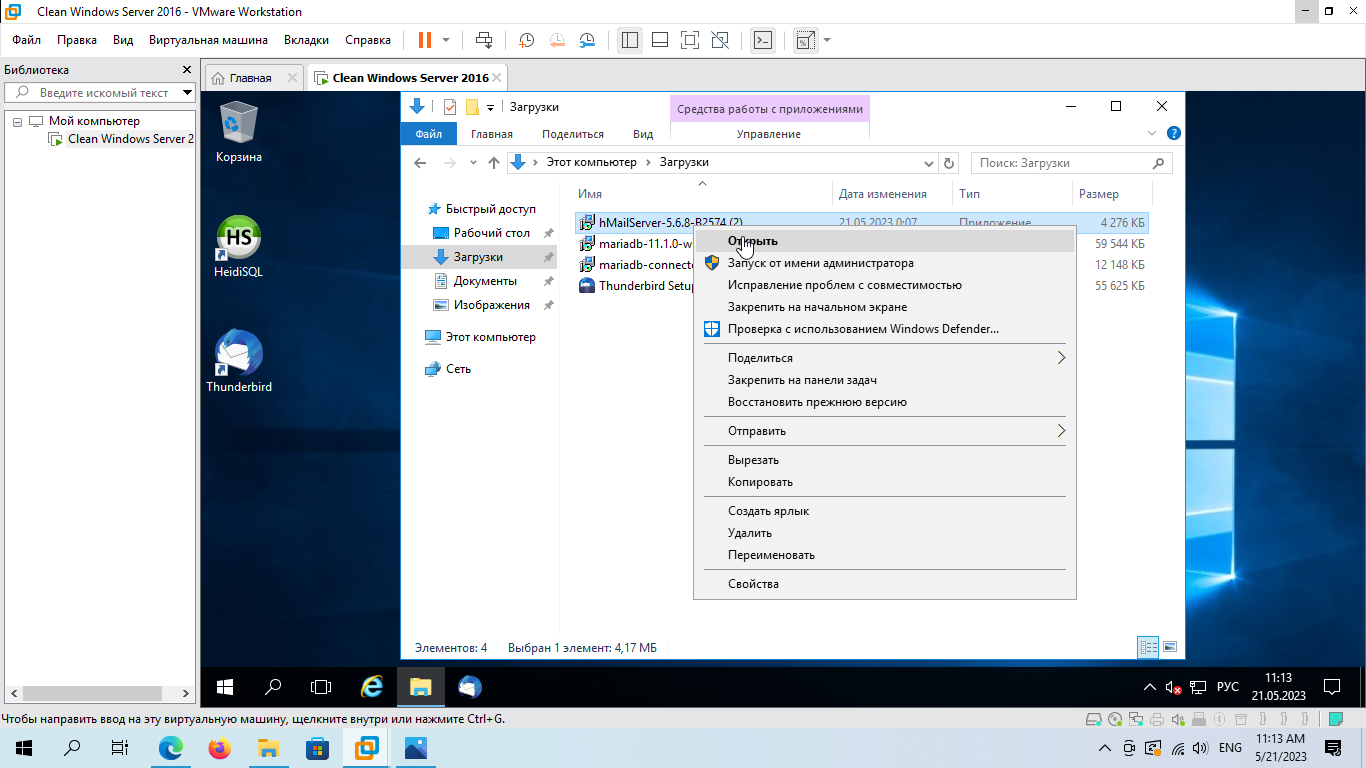
\includegraphics[width=\textwidth]{11_0046}
    \label{img:46}
    \caption{Начинаем установку \textit{hMailServer}}
  \end{figure}

  \begin{figure}[H]
    \centering
    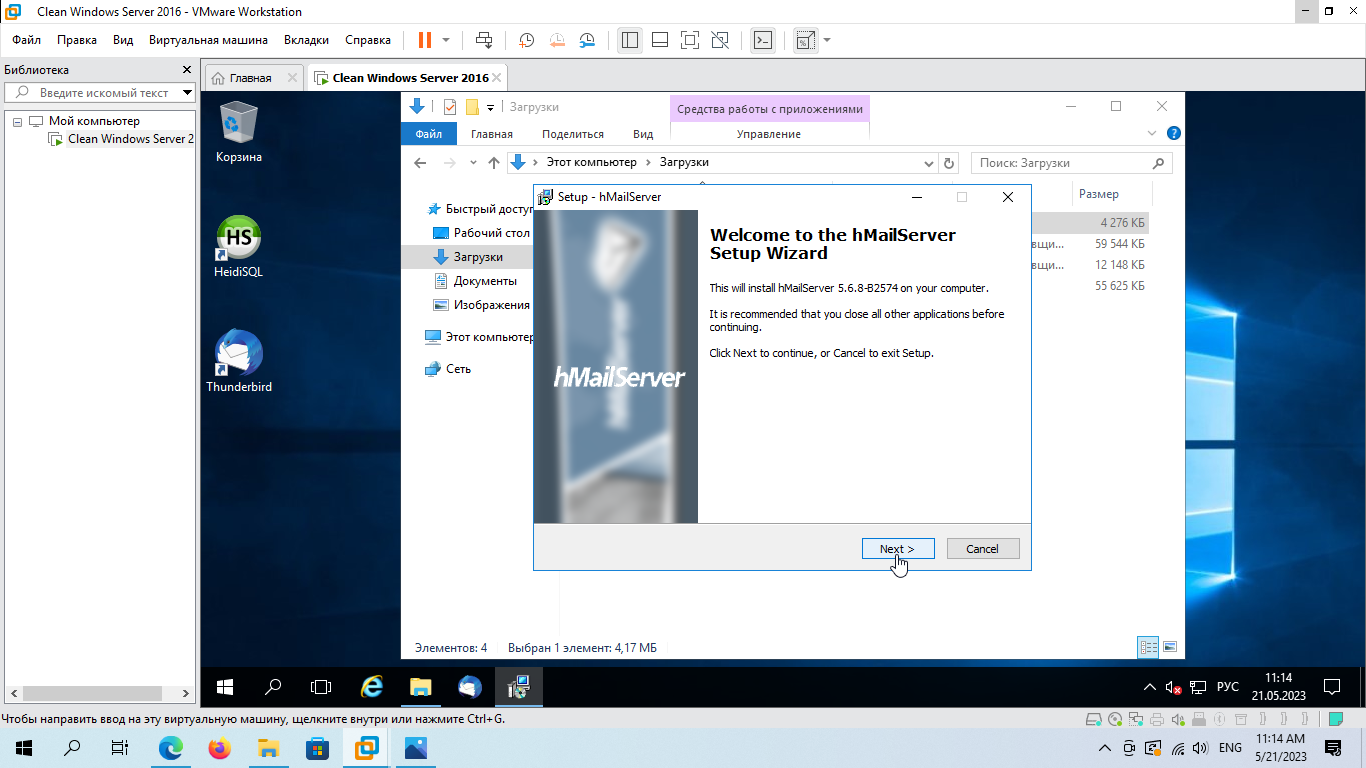
\includegraphics[width=\textwidth]{11_0047}
    \label{img:47}
    \caption{Далее}
  \end{figure}

  \begin{figure}[H]
    \centering
    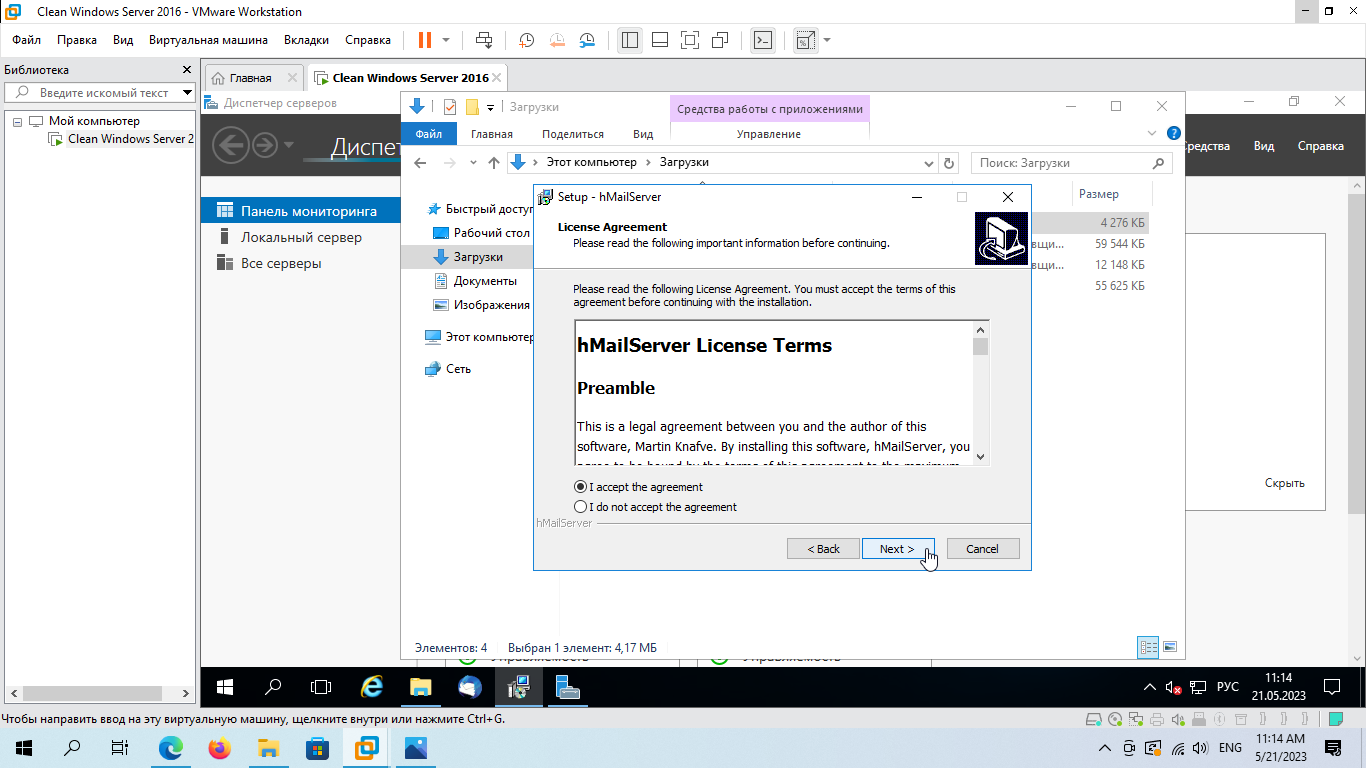
\includegraphics[width=\textwidth]{11_0048}
    \label{img:48}
    \caption{Принимаем условия использования данного ПО}
  \end{figure}

  \begin{figure}[H]
    \centering
    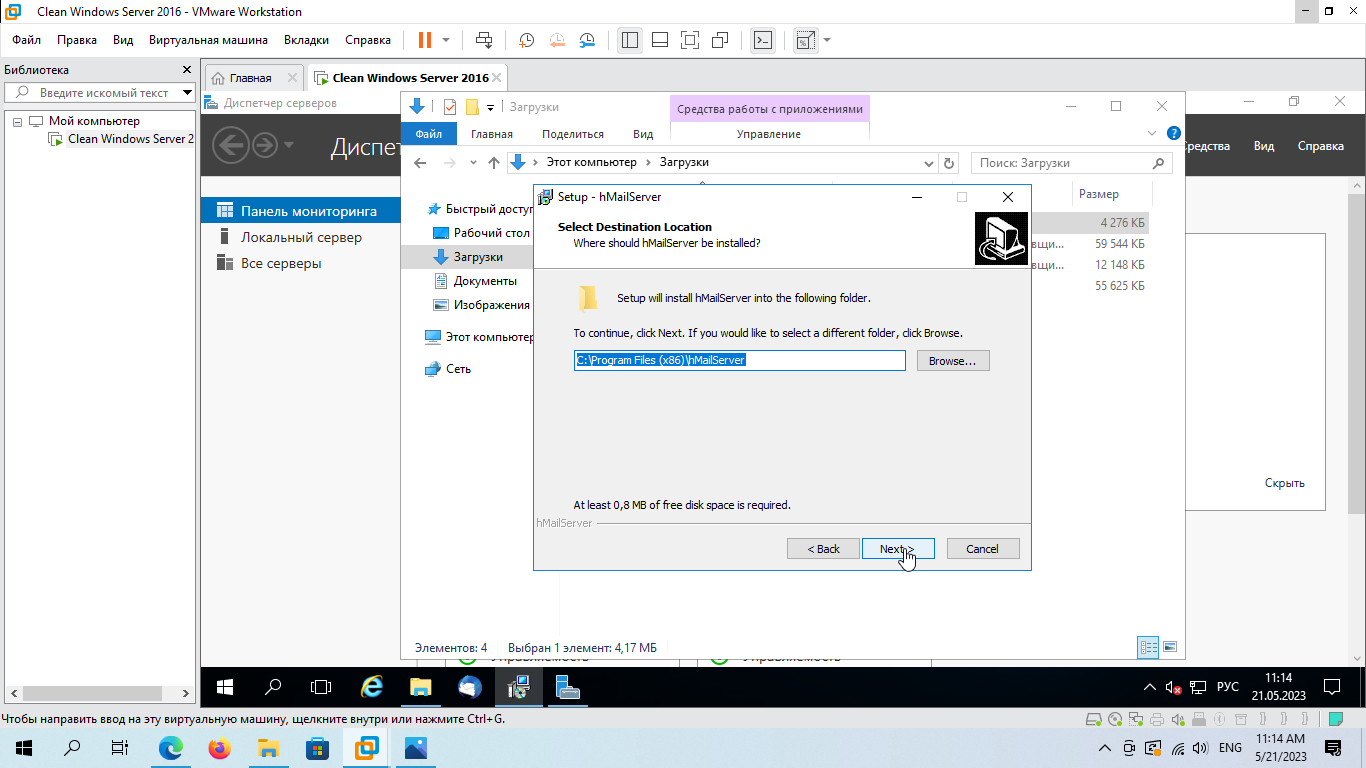
\includegraphics[width=\textwidth]{11_0049}
    \label{img:49}
    \caption{Не изменяем путь установки}
  \end{figure}

  \begin{figure}[H]
    \centering
    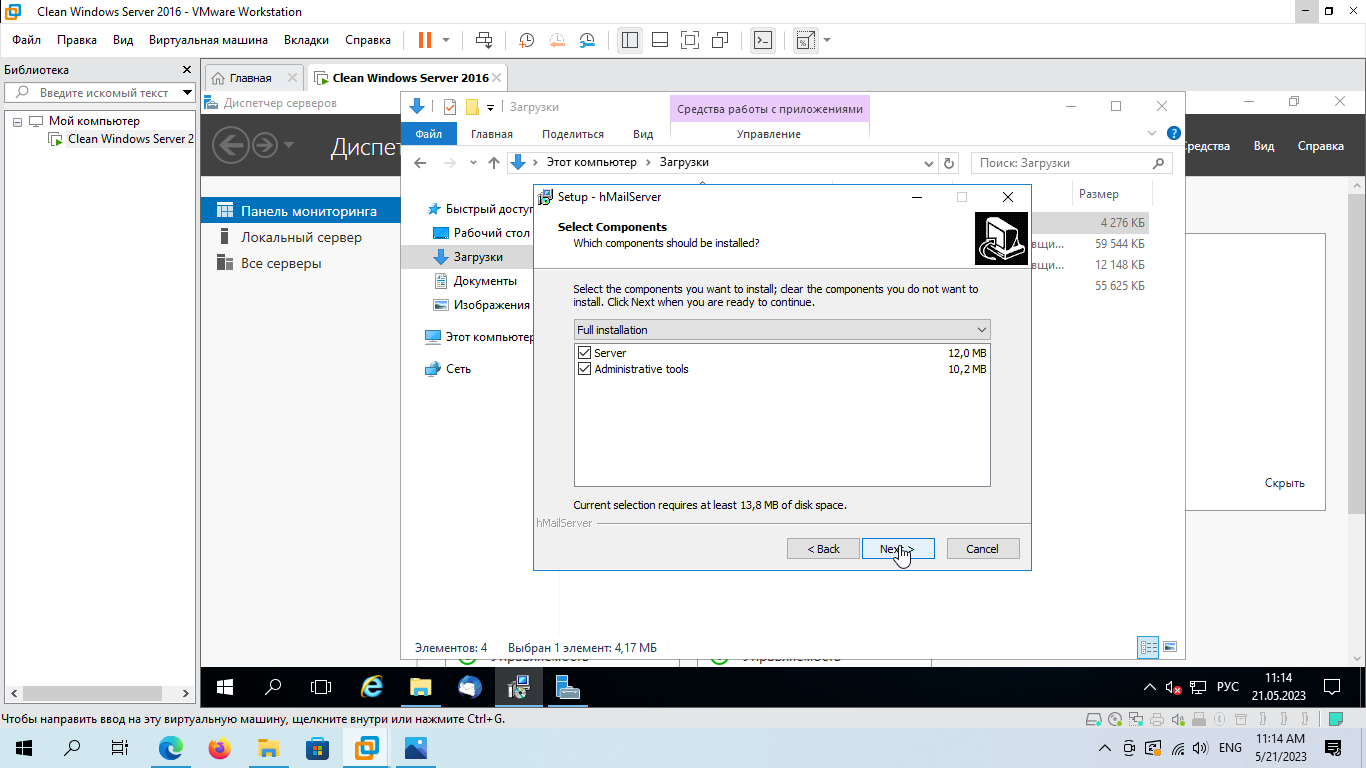
\includegraphics[width=\textwidth]{11_0050}
    \label{img:50}
    \caption{Устанавливаем все компоненты}
  \end{figure}

  \begin{figure}[H]
    \centering
    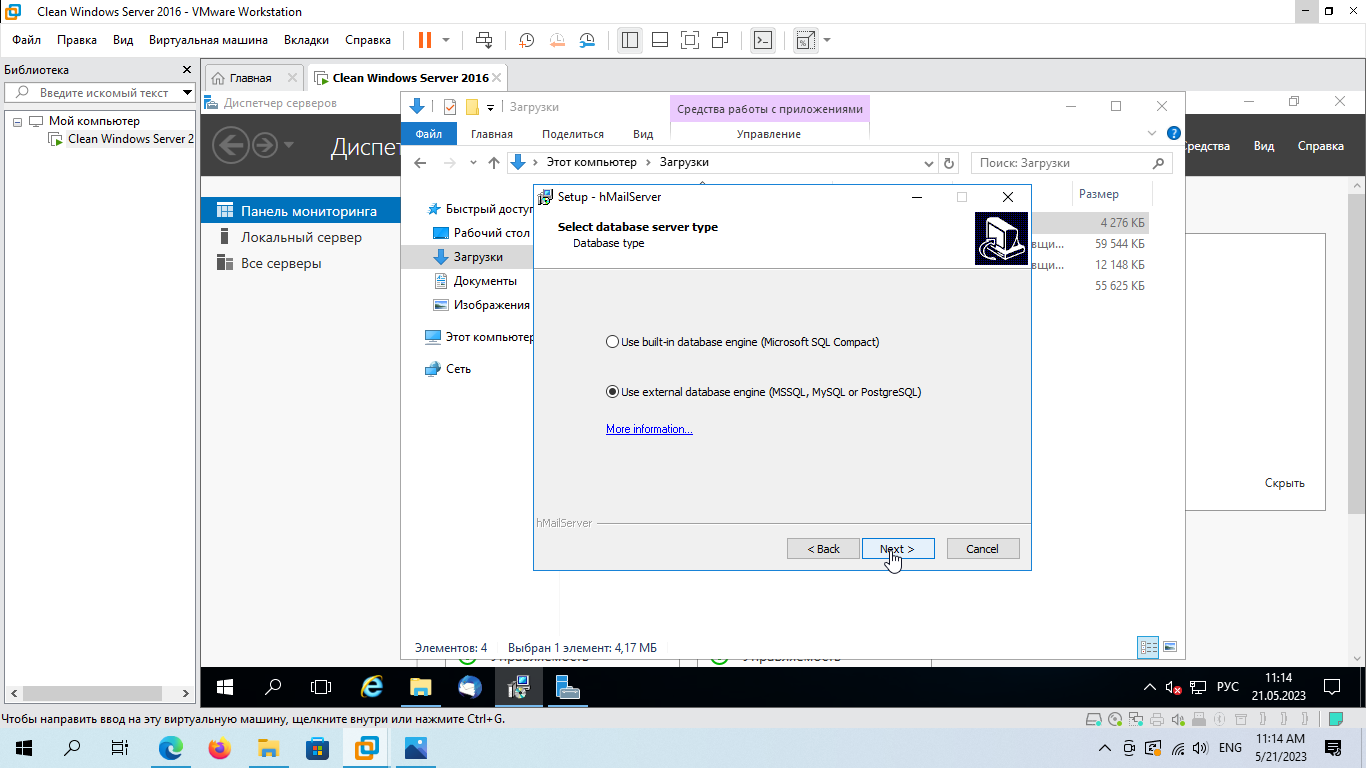
\includegraphics[width=\textwidth]{11_0051}
    \label{img:51}
    \caption{Необходима поддержка MySQL}
  \end{figure}

  \begin{figure}[H]
    \centering
    \includegraphics[width=\textwidth]{11_0052}
    \label{img:52}
    \caption{Далее}
  \end{figure}

  \begin{figure}[H]
    \centering
    \includegraphics[width=\textwidth]{11_0053}
    \label{img:53}
    \caption{Указываем пароль для доступа к настройкам сервера}
  \end{figure}

  \begin{figure}[H]
    \centering
    \includegraphics[width=\textwidth]{11_0054}
    \label{img:54}
    \caption{Установить}
  \end{figure}

  \begin{figure}[H]
    \centering
    \includegraphics[width=\textwidth]{11_0055}
    \label{img:55}
    \caption{Вводим заданный ранее пароль}
  \end{figure}

  \begin{figure}[H]
    \centering
    \includegraphics[width=\textwidth]{11_0056}
    \label{img:56}
    \caption{Теперь необходима настройка}
  \end{figure}

  \begin{figure}[H]
    \centering
    \includegraphics[width=\textwidth]{11_0057}
    \label{img:57}
    \caption{Создадим новую базу данных для сервера}
  \end{figure}

  \begin{figure}[H]
    \centering
    \includegraphics[width=\textwidth]{11_0058}
    \label{img:58}
    \caption{Указываем тип БД - MySQL}
  \end{figure}

  \begin{figure}[H]
    \centering
    \includegraphics[width=\textwidth]{11_0059}
    \label{img:59}
    \caption{Указываем данные для подключения к базе}
  \end{figure}

  \begin{figure}[H]
    \centering
    \includegraphics[width=\textwidth]{11_0060}
    \label{img:60}
    \caption{Указываем сервис - работающий сервер MySQL}
  \end{figure}

  \begin{figure}[H]
    \centering
    \includegraphics[width=\textwidth]{11_0061}
    \label{img:61}
    \caption{Далее}
  \end{figure}

  \begin{figure}[H]
    \centering
    \includegraphics[width=\textwidth]{11_0062}
    \label{img:62}
    \caption{Требуется библиотека для работы с MySQL}
  \end{figure}

  \begin{figure}[H]
    \centering
    \includegraphics[width=\textwidth]{11_0063}
    \label{img:63}
    \caption{Скопируем его из коннектора - libmariadb.dll}
  \end{figure}

  \begin{figure}[H]
    \centering
    \includegraphics[width=\textwidth]{11_0064}
    \label{img:64}
    \caption{И перенесем к файлам сервера с новым именем - libmysql.dll}
  \end{figure}

  \begin{figure}[H]
    \centering
    \includegraphics[width=\textwidth]{11_0065}
    \label{img:65}
    \caption{Далее}
  \end{figure}

  \begin{figure}[H]
    \centering
    \includegraphics[width=\textwidth]{11_0066}
    \label{img:66}
    \caption{Настройка БД для почтового сервера завершена}
  \end{figure}

  \begin{figure}[H]
    \centering
    \includegraphics[width=\textwidth]{11_0067}
    \label{img:67}
    \caption{В списке запущенный почтовый сервер}
  \end{figure}

  \begin{figure}[H]
    \centering
    \includegraphics[width=\textwidth]{11_0068}
    \label{img:68}
    \caption{Подключаемся к нему - указываем пароль}
  \end{figure}

  \begin{figure}[H]
    \centering
    \includegraphics[width=\textwidth]{11_0069}
    \label{img:69}
    \caption{Статус севреа - работает}
  \end{figure}

  \subsection{Настройка DNS}

  Чтобы почтовый клиент мог самостаятельно определять адрес 
  пчотовых серверов (для SMTP, IMAP, POP3), необходимо создать MX DNS запись:

  \begin{figure}[H]
    \centering
    \includegraphics[width=\textwidth]{11_0070}
    \label{img:70}
    \caption{Переходим к управлению DNS серверами}
  \end{figure}

  \begin{figure}[H]
    \centering
    \includegraphics[width=\textwidth]{11_0071}
    \label{img:71}
    \caption{Перейти к DNS}
  \end{figure}

  \begin{figure}[H]
    \centering
    \includegraphics[width=\textwidth]{11_0072}
    \label{img:72}
    \caption{Открываем диспетчер DNS}
  \end{figure}

  \begin{figure}[H]
    \centering
    \includegraphics[width=\textwidth]{11_0073}
    \label{img:73}
    \caption{Создадим новую зону прямого просмотра}
  \end{figure}

  \begin{figure}[H]
    \centering
    \includegraphics[width=\textwidth]{11_0074}
    \label{img:74}
    \caption{Тип зоны - основная}
  \end{figure}

  \begin{figure}[H]
    \centering
    \includegraphics[width=\textwidth]{11_0075}
    \label{img:75}
    \caption{Репликация - все компьютеры домена}
  \end{figure}

  \begin{figure}[H]
    \centering
    \includegraphics[width=\textwidth]{11_0076}
    \label{img:76}
    \caption{Указываем имя зоны - team9.local}
  \end{figure}

  \begin{figure}[H]
    \centering
    \includegraphics[width=\textwidth]{11_0077}
    \label{img:77}
    \caption{Разрешаем безопасные динамические обновления}
  \end{figure}

  \begin{figure}[H]
    \centering
    \includegraphics[width=\textwidth]{11_0078}
    \label{img:78}
    \caption{Готово - зона создана}
  \end{figure}

  \begin{figure}[H]
    \centering
    \includegraphics[width=\textwidth]{11_0079}
    \label{img:79}
    \caption{Создадим новую A запсиь}
  \end{figure}

  \begin{figure}[H]
    \centering
    \includegraphics[width=\textwidth]{11_0088}
    \label{img:88}
    \caption{Указываем IP адрес - текущий адрес сервера}
  \end{figure}

  \begin{figure}[H]
    \centering
    \includegraphics[width=\textwidth]{11_0089}
    \label{img:89}
    \caption{Узел добавлен}
  \end{figure}

  \begin{figure}[H]
    \centering
    \includegraphics[width=\textwidth]{11_0090}
    \label{img:90}
    \caption{Теперь создадим MX запись}
  \end{figure}

  \begin{figure}[H]
    \centering
    \includegraphics[width=\textwidth]{11_0091}
    \label{img:91}
    \caption{Привяжем ее к только что-созданной A записи}
  \end{figure}

  \begin{figure}[H]
    \centering
    \includegraphics[width=\textwidth]{11_0092}
    \label{img:92}
    \caption{Настроенная MX запись}
  \end{figure}

  \begin{figure}[H]
    \centering
    \includegraphics[width=\textwidth]{11_0093}
    \label{img:93}
    \caption{Необходимые записи созданы}
  \end{figure}

  \subsection{Создание пользователей}

  Создадим пользователей, которым позже присвоим email адреса:

  \begin{figure}[H]
    \centering
    \includegraphics[width=\textwidth]{11_0094}
    \label{img:94}
    \caption{Переходим к AD DS}
  \end{figure}

  \begin{figure}[H]
    \centering
    \includegraphics[width=\textwidth]{11_0095}
    \label{img:95}
    \caption{Перейти к AD DS}
  \end{figure}

  \begin{figure}[H]
    \centering
    \includegraphics[width=\textwidth]{11_0096}
    \label{img:96}
    \caption{Открываем список пользователей и компьютеров}
  \end{figure}

  \begin{figure}[H]
    \centering
    \includegraphics[width=\textwidth]{11_0097}
    \label{img:97}
    \caption{Создаем нового пользователя}
  \end{figure}

  \begin{figure}[H]
    \centering
    \includegraphics[width=\textwidth]{11_0098}
    \label{img:98}
    \caption{Указываем имя пользователя - User1}
  \end{figure}

  \begin{figure}[H]
    \centering
    \includegraphics[width=\textwidth]{11_0099}
    \label{img:99}
    \caption{Создаем для него пароль}
  \end{figure}

  \begin{figure}[H]
    \centering
    \includegraphics[width=\textwidth]{11_0100}
    \label{img:100}
    \caption{Повторяем создание пользователя}
  \end{figure}

  \begin{figure}[H]
    \centering
    \includegraphics[width=\textwidth]{11_0101}
    \label{img:101}
    \caption{Снова указываем имя}
  \end{figure}

  \begin{figure}[H]
    \centering
    \includegraphics[width=\textwidth]{11_0102}
    \label{img:102}
    \caption{И пароль для входа}
  \end{figure}

  \begin{figure}[H]
    \centering
    \includegraphics[width=\textwidth]{11_0103}
    \label{img:103}
    \caption{Пользователь добавлен}
  \end{figure}

  \subsection{Настройка почтового домена}

  \begin{figure}[H]
    \centering
    \includegraphics[width=\textwidth]{11_0104}
    \label{img:104}
    \caption{Добавим новый почтовый домен}
  \end{figure}

  \begin{figure}[H]
    \centering
    \includegraphics[width=\textwidth]{11_0135}
    \label{img:135}
    \caption{Укажем имя домена}
  \end{figure}

  \begin{figure}[H]
    \centering
    \includegraphics[width=\textwidth]{11_0136}
    \label{img:136}
    \caption{Перейдем к созданию почтовых адресов}
  \end{figure}

  \begin{figure}[H]
    \centering
    \includegraphics[width=\textwidth]{11_0137}
    \label{img:137}
    \caption{Добавим адрес user1@team9.local}
  \end{figure}

  \begin{figure}[H]
    \centering
    \includegraphics[width=\textwidth]{11_0138}
    \label{img:138}
    \caption{Привяжем его к пользователю User1}
  \end{figure}

  \begin{figure}[H]
    \centering
    \includegraphics[width=\textwidth]{11_0139}
    \label{img:139}
    \caption{Добавим еще один адрес}
  \end{figure}

  \begin{figure}[H]
    \centering
    \includegraphics[width=\textwidth]{11_0140}
    \label{img:140}
    \caption{Создаем адрес user2@team9.local}
  \end{figure}

  \begin{figure}[H]
    \centering
    \includegraphics[width=\textwidth]{11_0141}
    \label{img:141}
    \caption{Привязываем его к пользователю User2}
  \end{figure}

  Почтовый домен создан и настроен.

  \subsection{Настройка почтового клиента}

  Привяжем учетные записи пользователей почтового сервера к клиенту:

  \begin{figure}[H]
    \centering
    \includegraphics[width=\textwidth]{11_0142}
    \label{img:142}
    \caption{Указываем данные первого пользователя}
  \end{figure}

  \begin{figure}[H]
    \centering
    \includegraphics[width=\textwidth]{11_0143}
    \label{img:143}
    \caption{Почтовый сервер определилс автоматически - DNS работает корректно}
  \end{figure}

  \begin{figure}[H]
    \centering
    \includegraphics[width=\textwidth]{11_0144}
    \label{img:144}
    \caption{Принимаем риски - шифрование не настроенно}
  \end{figure}

  \begin{figure}[H]
    \centering
    \includegraphics[width=\textwidth]{11_0145}
    \label{img:145}
    \caption{Добавим вторую учетную запись}
  \end{figure}

  \begin{figure}[H]
    \centering
    \includegraphics[width=\textwidth]{11_0146}
    \label{img:146}
    \caption{Указываем данные второго пользователя}
  \end{figure}

  \begin{figure}[H]
    \centering
    \includegraphics[width=\textwidth]{11_0147}
    \label{img:147}
    \caption{Данные почтового сервера также определились автоматически}
  \end{figure}

  \subsection{Проверка работоспособности}

  Отправим письмо от пользователя User1 пользователю User2:

  \begin{figure}[H]
    \centering
    \includegraphics[width=\textwidth]{11_0148}
    \label{img:148}
    \caption{Указываем отправителя, получателя, тему и содержание письма и отправляем}
  \end{figure}

  \begin{figure}[H]
    \centering
    \includegraphics[width=\textwidth]{11_0149}
    \label{img:149}
    \caption{Письмо появилось в списке отправленных для User1}
  \end{figure}

  \begin{figure}[H]
    \centering
    \includegraphics[width=\textwidth]{11_0150}
    \label{img:150}
    \caption{Письмо появилось в списке входящих для User2}
  \end{figure}

  \newpage
  \section{Вывод}

  В ходе данной работы я научился устанавливать и настраивать MariaDB и почтовый
  сервер hMailServer.

\end{document}
